\chapter{数学分析：第一部分}

\begin{quote}
\emph{
现在，我们将开始一项重要工作：为微积分建立一个严谨的框架。前面关于逻辑与集合论的讨论已经提供了工具；第 1 章中的有序结构也揭示出一个关键事实——有理数虽然稠密，却并不完备。它们中间存在空隙，例如传说中的无理数 $\sqrt{2}$，它无法表示为两个整数之比。
}

\emph{
本章正是要面对这种不足。我们将构造实数系统，它是一块完备而连续的织物，用来填补这些空隙。它的基石是完备性公理，该公理保证有上界的集合具有精确的上确界，而这正是有理数致命缺失的性质。
}

\emph{
在这个不可动摇的基础上，我们将建立分析学的核心支柱：极限的精确定义、连续性的形式化定义，以及下一章中导数和积分的有力工具。这标志着从直观计算到深层理解的过渡，也就是从微积分走向分析学。
}
\end{quote}

\section{数系的扩张}
如果问数学分析的基础是什么，答案是明确的：实数公理。在这一部分中，我们将从 Peano 公理出发，形成自然数公理；随后出于实际需要，把自然数扩张为整数和有理数。接着，为了支撑微积分中的定理，我们构造实数和复数的公理体系。

在正式开始之前，需要先说明三个简单原则：
\begin{description}
    \item[动机原则（解决限制）] 每一次扩张都由某种运算在较小数系中并不总是可行这一需求推动。主要目标，是使新的数系对这种新运算具有\textbf{封闭性}。
    \item[嵌入原则（保持原有结构）] 原来的较小数系必须同构于新的较大数系中的某个子系统。这通常通过构造一个\textbf{单射嵌入}来实现，该嵌入保留原系统中的基本运算（如加法和乘法）以及性质。
    \item[最小性原则（“最小”的扩张）] 新数系应当是满足前两个原则的“最小”或“最经济”的扩张。它只应引入解决限制所必需的元素，而不应加入多余结构。
\end{description}

\subsection{Peano 公理与自然数}
Peano 公理用五条公理刻画自然数：
\begin{definition}[Peano 公理]
如果一个集合 $\mathbb{N}$ 满足下面性质（其中有一个“后继”函数 $S: \mathbb{N}\to \mathbb{N}$），则称 $\mathbb{N}$ 为\textbf{自然数集}：
\begin{enumerate}
    \item $0\in \mathbb{N}$。（零是自然数。）
    \item $\forall a\in \mathbb{N}(S(a)\in \mathbb{N})$。（如果 $a$ 是自然数，那么 $a$ 的后继也是自然数。）
    \item $\forall a\in \mathbb{N}(S(a)\ne 0)$。（零不是任何自然数的后继。）
    \item $\forall a,b\in \mathbb{N}(S(a)=S(b)\to a=b)$。（如果两个数的后继相等，那么这两个数本身相等。）
    \item $\forall K\subseteq \mathbb{N}[(0\in K\wedge \forall n(n\in K\to S(n)\in K))\to K=\mathbb{N}]$。（如果一个数集 $K$ 含有零，并且只要它含有某个数就也含有这个数的后继，那么每个自然数都在 $K$ 中。这就是\textbf{归纳公理}。）
\end{enumerate}
我们把 $a$ 的后继记作 $a+1$。
\end{definition}

自然数的定义与数学归纳法以及良序集概念有非常强的联系。实际上，在假定其他公理的前提下，它们在逻辑上是等价的。
\begin{itemize}
    \item Peano 公理保证数学归纳法成立（第五条公理就是数学归纳法）。
    \item Peano 公理保证良序原理成立。
\end{itemize}

下面证明良序原理（WOP）与数学归纳法（MI）之间的逻辑等价性。

\begin{proof}[数学归纳法推出良序原理]
\textbf{要证明：}自然数的每一个非空子集都有最小元。
反设存在一个非空子集 $A\subseteq \mathbb{N}$，但它\emph{没有}最小元。
定义另一个集合
\[
B=\{n\in \mathbb{N}\mid n<a\text{ 对所有 }a\in A\text{ 都成立}\}.
\]
也就是说，$B$ 是所有严格小于 $A$ 中每个元素的自然数组成的集合。

\textbf{基础情形：}$0\in B$ 吗？
如果 $0\notin B$，则存在某个 $a\in A$ 使得 $0\ge a$。由于 $a\in \mathbb{N}$，这推出 $a=0$。于是 $0\in A$。但零是最小的自然数，因此它就是 $A$ 的最小元，这与 $A$ 没有最小元的假设矛盾。所以 $0\in B$。

\textbf{归纳步骤：}假设 $k\in B$，证明 $S(k)\in B$。
归纳假设 $k\in B$ 的意思是，对所有 $a\in A$ 都有 $k<a$。
如果 $S(k)\notin B$，则存在某个 $a\in A$ 使得 $S(k)\ge a$。
结合假设 $k<a$ 与 $S(k)\ge a$，并且由于自然数是离散的，唯一可能是 $a=S(k)$。
于是 $S(k)\in A$。进一步地，所有小于 $S(k)$ 的数（例如 $k$）都在 $B$ 中，因此不在 $A$ 中，所以 $S(k)$ 会成为 $A$ 的最小元。
这与 $A$ 没有最小元的假设矛盾。因此 $S(k)\in B$。

\textbf{结论：}根据数学归纳法（第五条公理），$B=\mathbb{N}$。
由于 $A$ 非空，任取 $a\in A$。因为 $B=\mathbb{N}$，所以 $a\in B$。按照 $B$ 的定义，这意味着 $a<a$，矛盾。
最初关于 $A$ 没有最小元的假设必定为假。因此，自然数的每一个非空子集都有最小元。
\end{proof}

\begin{proof}[良序原理推出数学归纳法]
（这一部分留给读者练习。）
\end{proof}

\subsubsection*{势}
对有限集合来说，“数量”这个概念很清楚。但对于无限集合，我们应该怎样衡量集合的“大小”？
\begin{definition}[势 / 等势]
势是集合的一种内在性质。若两个集合 $A$ 和 $B$ 之间存在一个双射 $f:A\to B$，则称 $A$ 与 $B$ \textbf{等势}，或称它们有相同的\textbf{势}，记作 $A\approx B$ 或 $|A|=|B|$。
\end{definition}

\begin{definition}
对两个集合 $A$ 和 $B$，如果能够找到一个单射 $f:A\to B$，但不存在双射，则称集合 $A$ 严格小于集合 $B$，记作 $A\prec B$ 或 $|A|<|B|$。如果存在一个单射 $f:A\to B$，则记作 $A\preceq B$ 或 $|A|\le |B|$。
\end{definition}

\begin{theorem}[Schröder--Bernstein 定理]
如果 $A\preceq B$ 且 $B\preceq A$，那么 $A\approx B$。
\end{theorem}

\begin{definition}[可数集]
如果一个集合是有限集，或者它能够与自然数集 $\mathbb{N}$ 建立一一对应关系，则称该集合是\textbf{可数的}。如果一个集合是可数无限集，则把它的势定义为 $\aleph_0$（aleph-nought）。
\end{definition}

\begin{theorem}[Cantor 定理]
对每一个非空集合 $A$，都有 $A\prec \mathcal{P}(A)$。也就是说，$|A|<|\mathcal{P}(A)|$。
\end{theorem}
这说明不存在“最大的”无穷。

在第 2.3 节中，我们会知道实数集 $\mathbb{R}$ 的势为
\[
|\mathbb{R}|=|\mathcal{P}(\mathbb{N})|=2^{\aleph_0},
\]
它被称为\textbf{连续统}。

\paragraph{连续统假设（CH）}
有些读者可能会感兴趣：在 $\aleph_0$ 和 $2^{\aleph_0}$ 之间，是否还存在某种集合大小？连续统假设（CH）是一个著名猜想，它断言不存在集合 $S$ 使得
\[
\aleph_0<|S|<2^{\aleph_0}.
\]

那么，我们能判断它是真还是假吗？Kurt Gödel 和 Paul Cohen 已经证明，CH 在标准 ZFC 数学基础中是“不可判定”的。这意味着，利用公认的这些公理，既不能证明它为真，也不能证明它为假。这揭示了该系统的一种根本限制。

\subsection{整数与有理数}
为什么需要整数和有理数？为什么自然数还不够？
\begin{definition}[运算封闭性]
运算封闭性是指：当一个运算作用于某个集合的元素时，得到的结果仍然属于同一个集合。
\end{definition}
在自然数集 $\mathbb{N}$ 中，加法和乘法这样的运算是封闭的。但对减法（例如 $3-5=?$）和除法（例如 $3/5=?$）来说，$\mathbb{N}$ 本身并不够。因此，需要扩张数系。

\paragraph{整数 $\mathbb{Z}$ 的构造}
\begin{definition}
在 $\mathbb{N}\times \mathbb{N}$ 上定义关系 $R$：
\[
(a,b)R(c,d)\iff a+d=b+c.
\]
这是对 $a-b=c-d$ 的形式化表达。
\end{definition}

\begin{theorem}
关系 $R$ 是 $\mathbb{N}\times \mathbb{N}$ 上的等价关系。
\end{theorem}
\begin{proof}
（留给读者练习：检查自反性、对称性和传递性。）
\end{proof}

\begin{definition}[整数 $\mathbb{Z}$]
\textbf{整数集}，记作 $\mathbb{Z}$，是 $\mathbb{N}\times \mathbb{N}$ 关于等价关系 $R$ 的所有等价类构成的集合。我们把等价类 $[(a,b)]$ 记作 $a-b$。
\end{definition}

现在可以在 $\mathbb{Z}$ 上定义运算：
\begin{definition}[$\mathbb{Z}$ 上的运算]
\begin{itemize}
    \item \textbf{加法：} $[(a,b)]+[(c,d)]=[(a+c,b+d)]$；
    \item \textbf{相反数：} $-[(a,b)]=[(b,a)]$；
    \item \textbf{减法：} $[(a,b)]-[(c,d)]=[(a,b)]+(-[(c,d)])=[(a,b)]+[(d,c)]=[(a+d,b+c)]$。
\end{itemize}
\end{definition}
由于 $a,b,c,d\in \mathbb{N}$，并且 $\mathbb{N}$ 对加法封闭，所以 $a+d$ 和 $b+c$ 仍属于 $\mathbb{N}$。这意味着减法在整数中是封闭的。通过有序对从 $\mathbb{N}$ 构造 $\mathbb{Z}$，正是数系扩张原则的一个典型例子。

\paragraph{有理数 $\mathbb{Q}$ 的构造}
虽然 $\mathbb{Z}$ 对减法封闭，但它对除法并不封闭。因此，还需要把整数扩张为有理数。

\begin{definition}
令 $\mathbb{Z}^*=\mathbb{Z}-\{0\}$。在 $\mathbb{Z}\times \mathbb{Z}^*$ 上定义关系 $R$：
\[
(a,b)R(c,d)\iff ad=bc.
\]
这是对 $a/b=c/d$ 的形式化表达。
\end{definition}
显然，这个关系 $R$ 是一个等价关系。

\begin{definition}[有理数 $\mathbb{Q}$]
\textbf{有理数集}，记作 $\mathbb{Q}$，是 $\mathbb{Z}\times \mathbb{Z}^*$ 关于等价关系 $R$ 的所有等价类构成的集合。我们把等价类 $[(a,b)]$ 记作 $a/b$。
\end{definition}

\paragraph{有理数的稠密性}
有理数与整数相比，有一个非常不同的性质：有理数集是一个\textbf{稠密有序集}。在两个整数之间，我们并不总能找到另一个整数（例如 $1$ 和 $2$ 之间）；但在两个有理数之间，总能找到一个有理数作为中间值。
\begin{proof}
对两个有理数 $a$ 和 $b$，若 $a<b$，则它们的平均数 $m=(a+b)/2$ 仍是有理数，并且 $a<m<b$。因此，我们找到了位于二者之间的中间数。
\end{proof}
这一性质（$\mathbb{Q}$ 在 $\mathbb{R}$ 中的稠密性）对于构造和理解实数系统非常重要。在拓扑学中，$\mathbb{Q}$ 是 $\mathbb{R}$ 的一个可数稠密子集，这使得 $\mathbb{R}$ 成为可分空间。

\subsection{实数与复数}
有理数 $\mathbb{Q}$ 虽然稠密，但并不\emph{完备}。它们含有“空隙”。例如集合 $A=\{x\in \mathbb{Q}\mid x^2<2\}$ 在 $\mathbb{Q}$ 中有上界（如 $1.5$），但它在 $\mathbb{Q}$ \emph{内部}没有\emph{最小}上界。那个“数” $\sqrt{2}$ 缺失了。因此，我们构造实数 $\mathbb{R}$ 来填补这些空隙。

\subsubsection{用 Dedekind 分割构造实数}

\begin{definition}[Dedekind 分割]
\textbf{Dedekind 分割}是 $\mathbb{Q}$ 的两个子集组成的有序对 $(A,B)$，满足：
\begin{enumerate}
    \item $A$ 与 $B$ 非空，并且构成 $\mathbb{Q}$ 的一个划分，即 $A\cup B=\mathbb{Q}$ 且 $A\cap B=\emptyset$；
    \item $A$ 中每个元素都小于 $B$ 中每个元素；
    \item $A$ 没有最大元。
\end{enumerate}
集合 $A$ 称为\textbf{下类}，$B$ 称为\textbf{上类}。一个实数被定义为一个 Dedekind 分割。
\end{definition}

例如，实数 $\sqrt{2}$ 可以由下面的分割表示：
\begin{itemize}
    \item $A=\{x\in \mathbb{Q}\mid x<0\text{ 或 }x^2<2\}$；
    \item $B=\{x\in \mathbb{Q}\mid x>0\text{ 且 }x^2>2\}$。
\end{itemize}

\begin{definition}[实数上的序]
对两个实数 $\alpha=(A_1,B_1)$ 和 $\beta=(A_2,B_2)$，若 $A_1\subset A_2$（真包含），则定义 $\alpha<\beta$。若 $A_1=A_2$，则定义 $\alpha=\beta$。
\end{definition}

\begin{definition}[实数加法]
设 $\alpha=(A_1,B_1)$ 和 $\beta=(A_2,B_2)$ 为实数，定义：
\begin{itemize}
    \item $A=\{a_1+a_2\mid a_1\in A_1, a_2\in A_2\}$；
    \item $B=\mathbb{Q}\setminus A$。
\end{itemize}
于是 $\alpha+\beta$ 被定义为分割 $(A,B)$。
\end{definition}

\begin{definition}[正实数的乘法]
对正实数 $\alpha=(A_1,B_1)$ 和 $\beta=(A_2,B_2)$（这里“正”指它们的下类中含有某些正有理数），定义：
\begin{itemize}
    \item $A=\{a_1a_2\mid a_1\in A_1,a_2\in A_2,a_1>0,a_2>0\}\cup \{q\in \mathbb{Q}\mid q\le 0\}$；
    \item $B=\mathbb{Q}\setminus A$。
\end{itemize}
于是 $\alpha\cdot\beta$ 被定义为分割 $(A,B)$。对于其他符号组合，需要相应调整定义。
\end{definition}

\begin{definition}[加法逆元]
对实数 $\alpha=(A,B)$，定义它的加法逆元 $-\alpha$：
\begin{itemize}
    \item $A'=\{-b\mid b\in B,\ b\text{ 不是 }B\text{ 的最小元}\}$；
    \item $B'=\mathbb{Q}\setminus A'$。
\end{itemize}
于是 $-\alpha=(A',B')$。
\end{definition}

这些运算使 $\mathbb{R}$ 成为一个有序域。非零元素的乘法逆元也可以类似定义。

现在可以定义分析学中的基本概念：

\begin{definition}[上界]
设 $S\subseteq \mathbb{R}$。如果对所有 $s\in S$ 都有 $s\le u$，则称 $u$ 是 $S$ 的一个\textbf{上界}。如果对所有 $s\in S$ 都有 $l\le s$，则称 $l$ 是 $S$ 的一个\textbf{下界}。
\end{definition}

\begin{definition}[上确界]
$S$ 的\textbf{上确界}（或\textbf{最小上界}），记作 $\sup S$，是 $S$ 的最小上界。也就是说：
\begin{enumerate}
    \item 对所有 $s\in S$，有 $s\le \sup S$。（$\sup S$ 是上界。）
    \item 如果 $v$ 是 $S$ 的任意一个上界，则 $\sup S\le v$。（它是\emph{最小}上界。）
\end{enumerate}
\textbf{下确界}（或\textbf{最大下界}）的定义类似，记作 $\inf S$。
\end{definition}

\begin{theorem}[完备性公理]
$\mathbb{R}$ 的每一个非空且有上界的子集，都在 $\mathbb{R}$ 中有上确界。
\end{theorem}
下确界的情形类似：$\mathbb{R}$ 的每一个非空且有下界的子集，都在 $\mathbb{R}$ 中有下确界。

\begin{proof}
在 Dedekind 分割构造中，一个有界实数集 $S$ 的上确界可以由 $S$ 中所有元素的下类之并给出。更准确地说，如果 $S=\{\alpha_i=(A_i,B_i)\}$ 有上界，则
\[
\sup S=\left(\bigcup_i A_i,\mathbb{Q}\setminus \bigcup_i A_i\right).
\]
这个有序对构成一个 Dedekind 分割，并且满足上确界的定义。
\end{proof}

完备性公理是分析学的基础，它把 $\mathbb{R}$ 与 $\mathbb{Q}$ 区分开来。它保证 Cauchy 列的极限存在，连续函数在闭区间上能够取得最大值和最小值，也保证许多其他关键性质。从现在开始，我们可以说每个收敛的实数列都收敛到某个实数。这正是\textbf{完备性公理}在分析学中的含义。

\begin{definition}[Archimedean 性质]
实数满足\textbf{Archimedean 性质}：对任意 $x\in \mathbb{R}$，存在自然数 $n$ 使得 $n>x$。等价地，对任意 $\epsilon>0$，存在 $n\in \mathbb{N}$ 使得 $1/n<\epsilon$。
\end{definition}

\begin{theorem}[有理数的稠密性]
任意两个不同实数之间，都存在一个有理数。也就是说，$\mathbb{Q}$ 在 $\mathbb{R}$ 中\textbf{稠密}。
\end{theorem}

虽然 $\mathbb{R}$ 解决了 $\mathbb{Q}$ 的完备性问题，但它并不是\textbf{代数闭}的。存在一些实系数多项式方程没有实数解，例如 $x^2+1=0$。这推动我们进一步扩张到复数。

\paragraph{复数的构造}

现在，我们构造一种新的数域，它是人类历史上曾认识到的最大的常用数域。

\begin{definition}[复数]
\textbf{复数集}，记作 $\mathbb{C}$，由所有形如 $a+bi$ 的表达式组成，其中 $a,b\in \mathbb{R}$，而 $i$ 是满足 $i^2=-1$ 的\textbf{虚数单位}。对 $z=a+bi\in \mathbb{C}$：
\begin{itemize}
    \item $a$ 称为\textbf{实部}，记作 $\Re(z)$；
    \item $b$ 称为\textbf{虚部}，记作 $\Im(z)$。
\end{itemize}
\end{definition}

两个复数 $a+bi$ 和 $c+di$ 相等，当且仅当 $a=c$ 且 $b=d$。

\begin{definition}[复数运算]
对复数 $z=a+bi$ 和 $w=c+di$，定义：
\begin{itemize}
    \item \textbf{加法：}$z+w=(a+c)+(b+d)i$；
    \item \textbf{乘法：}$zw=(ac-bd)+(ad+bc)i$。
\end{itemize}
\end{definition}

在这些运算下，$\mathbb{C}$ 构成一个域。实数集 $\mathbb{R}$ 可以被看作 $\mathbb{C}$ 中的子集 $\{a+0i:a\in \mathbb{R}\}$。

\begin{definition}[复共轭与模]
对 $z=a+bi\in \mathbb{C}$：
\begin{itemize}
    \item \textbf{复共轭}为 $\bar z=a-bi$；
    \item \textbf{模}（或绝对值）为 $|z|=\sqrt{a^2+b^2}$。
\end{itemize}
\end{definition}

\begin{theorem}[共轭与模的性质]
对 $z,w\in \mathbb{C}$，有：
\begin{enumerate}
    \item $\overline{z+w}=\bar z+\bar w$；
    \item $\overline{zw}=\bar z\cdot \bar w$；
    \item $z\bar z=|z|^2$；
    \item $|zw|=|z||w|$；
    \item $|z+w|\le |z|+|w|$（三角不等式）。
\end{enumerate}
\end{theorem}

\begin{theorem}[代数基本定理]
每一个复系数非常数多项式至少有一个复根。等价地，$\mathbb{C}$ 是代数闭的。
\end{theorem}

这个定理非常深刻：我们最初是为了求解方程 $x^2+1=0$ 而把 $\mathbb{R}$ 扩张为 $\mathbb{C}$，但最终得到的数系中，每一个多项式方程都有解。

\begin{definition}[复数的极坐标形式]
任意非零复数 $z=a+bi$ 都可以写成\textbf{极坐标形式}
\[
z=r(\cos\theta+i\sin\theta),
\]
其中 $r=|z|>0$ 是模，$\theta$ 是 $z$ 的\textbf{辐角}，满足 $\tan\theta=b/a$。
\end{definition}

利用 Euler 公式 $e^{i\theta}=\cos\theta+i\sin\theta$，可以写作 $z=re^{i\theta}$。

\begin{theorem}[De Moivre 定理]
对任意整数 $n$ 和复数 $z=r(\cos\theta+i\sin\theta)$，有
\[
z^n=r^n(\cos(n\theta)+i\sin(n\theta)).
\]
\end{theorem}

这个定理简化了复数幂与复数根的计算。

复数为数学、物理和工程中的许多领域提供了强大的框架。它们使我们能够：
\begin{itemize}
    \item 求解所有多项式方程；
    \item 用复指数表示周期现象；
    \item 在电气工程中分析信号与系统；
    \item 研究流体力学和电磁学；
    \item 建立量子力学的数学基础。
\end{itemize}

\section{数列极限与实数的性质}

完成实数的内容之后，我们现在进入数学分析的核心：\textbf{极限}。为什么说极限是数学分析的核心概念？在接下来的内容中会看到，几乎所有概念都与极限存在某种联系。可以说，极限是许多理论的基础。而极限语言体现的是一种动态的、趋近的、严谨的数学思维方式。现在开始。

\subsection{定义与基本性质}

\subsubsection{极限的定义}

\begin{definition}[数列极限]
如果数列 $\{a_n\}$ 收敛到实数 $A$，意思是：对任意 $\epsilon>0$，存在整数 $N$，使得当 $n\ge N$ 时，有 $|a_n-A|<\epsilon$。数 $A$ 称为该数列的极限，记作
\[
\lim_{n\to \infty}a_n=A.
\]
\end{definition}
朴素地说，如果数列 $\{a_n\}$ 是一个\textbf{收敛数列}，且 $A$ 是它的极限，那么 $a_n$ 的值会任意接近某个有限数 $A$。只要取足够大的 $n$，就可以让 $a_n$ 任意接近收敛值 $A$。

用更常见的语言来说，如果在实数轴上取一个以 $a$ 为中心、以 $\epsilon$ 为半径的开区间 $(a-\epsilon,a+\epsilon)$，我们称这种区间为邻域，记作 $O(a,\epsilon)$：
\[
O(a,\epsilon)=\{x\mid a-\epsilon<x<a+\epsilon\}.
\]
这个定义的意思是，在某一项之后，所有 $a_n$ 都落在 $O(a,\epsilon)$ 中。由于这个邻域可以任意缩小，数列最终就收敛到 $a$。

相反，如果一个数列 $\{a_n\}$ 不收敛，我们就称它为\textbf{发散数列}。严格地说，如果对所有 $\epsilon>0$、$N\in \mathbb{N}^*$ 以及 $A\in \mathbb{R}$，总存在至少一个 $n_0$ 使得 $|a_{n_0}-A|>\epsilon$，那么该数列不收敛。

对于收敛到 $0$ 的数列，我们称它们为\textbf{无穷小}。

\begin{remark}
谈论无穷小时，我们讨论的是一个数列，而不是一个单独的数。需要清楚：无穷小不是一个数。
\end{remark}

\subsubsection{极限的性质}

定义极限之后，下面来看它的一些性质。

\begin{theorem}[极限的唯一性]
收敛数列的极限必定唯一。
\end{theorem}
\begin{proof}
假设存在数列 $\{a_n\}$ 同时收敛到两个不同的值 $a$ 和 $b$，且 $a\ne b$。根据极限定义：
\[
\forall \epsilon>0,\exists N_1,n>N_1:|x_n-a|<\epsilon/2,
\]
\[
\forall \epsilon>0,\exists N_2,n>N_2:|x_n-b|<\epsilon/2.
\]
取 $N=\max\{N_1,N_2\}$。由三角不等式，对所有 $n>N$ 有
\[
|a-b|=|a-x_n+x_n-b|\le |x_n-a|+|x_n-b|<\epsilon.
\]
由于 $\epsilon$ 可以任意接近 $0$，所以 $a=b$。
\end{proof}

\begin{theorem}
收敛数列必定有界。
\end{theorem}
\begin{remark}
但是其逆命题并不总是成立。有界数列未必收敛。

例如 $a_n=(-1)^n$，数列 $\{a_n\}$ 被限制在 $-1$ 和 $1$ 之间，但它并不收敛到任何值。

以后我们可以加入更强的条件，使 $\{a_n\}$ 收敛。后文会介绍。
\end{remark}

\begin{proof}
设 $\{a_n\}$ 是收敛数列，极限为 $a$。根据极限定义，取 $\epsilon=1$，于是存在 $N$，使得对所有 $n>N$，$|x_n-a|<1$，即 $a-1<x_n<a+1$。

令
\[
m=\min\{a_1,a_2,\dots,a_N,a-1\},\quad M=\max\{a_1,a_2,\dots,a_N,a+1\}.
\]
则对所有 $n$，有 $m\le x_n\le M$，因此数列 $\{x_n\}$ 有界。
\end{proof}

\begin{theorem}[保序性]
设有两个数列 $\{x_n\}$ 和 $\{y_n\}$，它们分别收敛到 $a$ 和 $b$，且 $a<b$。则存在 $N$，使得对所有 $n>N$，都有 $x_n<y_n$。
\end{theorem}

\begin{proof}
设两个数列 $\{x_n\}$ 和 $\{y_n\}$ 分别收敛到 $a$ 与 $b$。先考虑 $a>b$ 的情形。
根据极限定义，取 $\epsilon=(a-b)/2$，则
\[
\exists N_1,\forall n>N_1, |x_n-a|<\epsilon,
\]
\[
\exists N_2,\forall n>N_2, |y_n-b|<\epsilon.
\]
于是 $x_n>(a+b)/2>y_n$。取 $N=\max\{N_1,N_2\}$，就有 $\forall n>N,x_n>y_n$。因此，极限具有保序性。
\end{proof}

\newpage

\begin{theorem}[极限的运算法则]
设存在两个极限
\[
\lim_{n\to \infty}x_n=a,\quad \lim_{n\to \infty}y_n=b.
\]
则有：
\begin{itemize}
    \item 对任意常数 $\alpha,\beta$，$\lim_{n\to \infty}(\alpha x_n+\beta y_n)=\alpha a+\beta b$；
    \item $\lim_{n\to \infty}x_ny_n=ab$；
    \item $\lim_{n\to \infty}\left(\frac{x_n}{y_n}\right)=\frac{a}{b}$，其中 $b\ne 0$。
\end{itemize}
\end{theorem}
建议读者自行完成上述证明。

在定义了收敛数列和它的一些基本性质之后，我们现在定义一种特殊的不收敛数列：\textbf{无穷大}。

\subsubsection{无穷大}

\begin{definition}[无穷大]
设有数列 $\{x_n\}$。如果对每个给定的 $G>0$，都能找到 $N\in \mathbb{N}$，使得对所有 $n>N$，都有 $|x_n|>G$，则称数列 $\{x_n\}$ 为无穷大，记作
\[
\lim_{n\to \infty}x_n=\infty.
\]
\end{definition}

就像无穷小一样，无穷大也是一个数列，而不是一个数。但在某些情形下，我们会像处理数一样处理它。

如果某个无穷大数列从某一项起始终为正，就称它为\textbf{正无穷大}。负无穷大也可以类似定义。我们特别记作
\[
\lim_{n\to \infty}a_n=+\infty,\quad (\lim_{n\to \infty}a_n=-\infty).
\]

\begin{theorem}
无穷大与无穷小之间有特殊关系：数列 $\{x_n\}$（$x_n\ne 0$）是无穷大，当且仅当 $\{1/x_n\}$ 是无穷小。
\end{theorem}
用极限定义即可证明该定理，这里略去。

\begin{theorem}
设 $\{x_n\}$ 是无穷大。如果当 $n>N_0$ 时，有 $|y_n|\ge \delta>0$，则 $\{x_ny_n\}$ 是无穷大。
\end{theorem}

\begin{inference}
设 $\{x_n\}$ 是无穷大，且 $\lim_{n\to \infty}y_n=b\ne 0$，则 $\{x_ny_n\}$ 与 $\{x_n/y_n\}$ 都是无穷大。
\end{inference}

\subsubsection{Stolz 定理}

借助极限定义，可以用代数技巧和极限定义计算各种极限。但面对某些形式，例如 $\frac{0}{0}$ 和 $\frac{\infty}{\infty}$，处理起来尤其困难。下面要介绍的 \textbf{Stolz 定理}可以在某些场合让这类问题变得简单。

\begin{definition}[递增数列]
如果数列 $\{x_n\}$ 满足 $x_n\le x_{n+1}$，$n=1,2,3,\cdots$，则称它为\textbf{单调递增数列}。类似地，如果 $\forall n\in \mathbb{N}$，$x_n<x_{n+1}$，则称它为\textbf{严格单调递增数列}。
\end{definition}

\begin{theorem}
设 $\{y_n\}$ 是\textbf{严格单调递增的正无穷大}，且
\[
\lim_{n\to \infty}\frac{x_n-x_{n-1}}{y_n-y_{n-1}}=a.
\]
那么
\[
\lim_{n\to \infty}\frac{x_n}{y_n}=a.
\]
\end{theorem}

\begin{proof}
先考虑 $a=0$ 的情形。
因为 $\lim_{n\to \infty}\frac{x_n-x_{n-1}}{y_n-y_{n-1}}=0$，根据极限定义，有
\[
\forall \epsilon>0,\exists N_1,\forall n>N_1:|x_n-x_{n-1}|<\epsilon(y_n-y_{n-1}).
\]
由于 $\{y_n\}$ 是无穷大，显然可以令 $y_{N_1}>0$。对上面的不等式从 $N_1$ 到 $n$ 累加，得到
\[
|x_n-x_{N_1}|\le |x_n-x_{n-1}|+|x_{n-1}-x_{n-2}|+\cdots+|x_{N_1+1}-x_{N_1}|
\]
\[
<\epsilon(y_n-y_{n-1})+\cdots+\epsilon(y_{N_1+1}-y_{N_1})=\epsilon(y_n-y_{N_1}).
\]
两边同除以 $y_n$，得到
\[
\left|\frac{x_n}{y_n}-\frac{x_{N_1}}{y_n}\right|\le \epsilon\left(1-\frac{y_{N_1}}{y_n}\right)\le \epsilon.
\]
对于固定的 $N_1$，可取 $N>N_1$，使得对所有 $n>N$，有 $|x_{N_1}/y_n|<\epsilon$。于是
\[
\left|\frac{x_n}{y_n}\right|<\epsilon+\left|\frac{x_{N_1}}{y_n}\right|<2\epsilon.
\]

若 $a$ 是有限值且 $a\ne 0$，令 $x'_n=x_n-ay_n$，利用上面的证明即可得到结论。

当 $a=+\infty$ 时，考虑 $x_n/y_n$ 的倒数，类似地也不难得到结论。
\end{proof}

以后还会遇到一个与 \textbf{Stolz 定理}非常相似的结果，即\textbf{L'Hôpital 法则}。函数与数列之间存在许多相似之处，后续章节还会看到更多例子。

\subsection{收敛准则与实数系统的性质}

在讨论导数、积分等更高级的分析概念之前，必须先牢固建立实数系统 $\mathbb{R}$ 的一个基本性质：\textbf{完备性}。正是这一性质把实数 $\mathbb{R}$ 与有理数 $\mathbb{Q}$ 区分开来，并成为分析学中所有重要定理的基石。

\subsubsection{实数系统的完备性}

实数系统的完备性可以用若干等价方式表达。这里先回顾一下。（证明见第 2.1.3 节。）

\begin{theorem}[完备性公理]
\label{thm:completeness_cn}
$\mathbb{R}$ 的每一个非空且有上界的子集，都在 $\mathbb{R}$ 中有上确界。
\end{theorem}

这个公理看似简单，却直接导出了分析学中的第一个重要收敛准则。

\subsubsection{单调收敛定理}

前面已经定义了单调递增数列。完备性公理保证：有界的单调数列必定收敛。

\begin{theorem}[单调收敛定理]
\label{thm:mct_cn}
有界的单调数列（递增或递减）必定收敛。
\begin{itemize}
    \item (i) 如果 $\{x_n\}$ 单调递增且有上界，则 $\lim_{n\to \infty}x_n=\sup\{x_n\}$。
    \item (ii) 如果 $\{x_n\}$ 单调递减且有下界，则 $\lim_{n\to \infty}x_n=\inf\{x_n\}$。
\end{itemize}
\end{theorem}

\begin{proof}
证明 (i)；(ii) 的证明类似。
设 $\{x_n\}$ 是单调递增且有上界的数列。令 $S=\{x_n\mid n\in \mathbb{N}\}$ 为其所有项构成的集合。
由假设，$S$ 非空且有上界。
根据完备性公理，$S$ 必有上确界。令 $a=\sup S$。

下面证明 $\lim_{n\to \infty}x_n=a$。
根据极限定义，需要证明
\[
\forall \epsilon>0,\exists N\in \mathbb{N},\forall n>N:|x_n-a|<\epsilon.
\]
这等价于 $a-\epsilon<x_n<a+\epsilon$。

\begin{enumerate}
    \item 首先，根据上确界定义，$a$ 是 $S$ 的上界，因此对所有 $n$，$x_n\le a$。显然有 $x_n<a+\epsilon$。
    \item 接着考虑 $a-\epsilon$。由于 $a$ 是\textit{最小}上界，$a-\epsilon$ 小于 $a$，所以它\textit{不可能}是 $S$ 的上界。
    \item 因为 $a-\epsilon$ 不是上界，所以存在某个 $x_N\in S$ 使得 $x_N>a-\epsilon$。
    \item 由于 $\{x_n\}$ 单调递增，对任意 $n>N$，有 $x_n\ge x_N$。
    \item 结合以上各点，得到
    \[
    \forall n>N:a-\epsilon<x_N\le x_n\le a<a+\epsilon.
    \]
    因而 $\forall n>N:|x_n-a|<\epsilon$。
\end{enumerate}
所以 $\lim_{n\to \infty}x_n=a$。
\end{proof}

\subsubsection{Cauchy 收敛准则}

单调收敛定理很有力，但它要求数列单调。对一般情形，我们需要一种不依赖单调性、也不要求事先知道极限值的收敛判据。这就是 Cauchy 准则。

\begin{definition}[Cauchy 数列]
如果数列 $\{x_n\}$ 满足
\[
\forall \epsilon>0,\exists N\in \mathbb{N},\forall m,n>N:|x_m-x_n|<\epsilon,
\]
则称它为\textbf{Cauchy 数列}。直观地说，Cauchy 数列的“尾部”各项会彼此任意接近。
\end{definition}

在证明 Cauchy 准则之前，需要一个关键引理，它本身也是完备性公理的重要结果。我们还需要引入一个关键概念：\textbf{子列}，从而说明 Bolzano--Weierstrass 定理。

\begin{definition}[子列]
设有一个严格单调递增的自然数列 $\{k_n\}$ 和一个“母数列” $\{a_n\}$：
\[
k_1,k_2,\cdots,k_n,k_{n+1},\cdots.
\]
如果 $\forall i\in \mathbb{N}$，$k_i\in \mathbb{N}$，则称
\[
a_{k_1},a_{k_2},a_{k_3},\cdots,a_{k_n},a_{k_{n+1}},\cdots
\]
为数列 $\{a_n\}$ 的一个子列。
\end{definition}

\begin{theorem}[Bolzano--Weierstrass 定理]
\label{thm:bw_cn}
$\mathbb{R}$ 中的每一个有界数列都含有一个收敛子列。
\end{theorem}

\begin{proof}
（证明概要）设 $\{x_n\}$ 是有界数列，它的所有项都位于闭区间 $[a,b]$ 中。
把 $[a,b]$ 二等分为 $[a,(a+b)/2]$ 与 $[(a+b)/2,b]$。至少有一个子区间包含 $\{x_n\}$ 的无穷多项。选择这样的区间，记作 $I_1=[a_1,b_1]$。
接着二等分 $I_1$，再次选择一个包含无穷多项的子区间，记作 $I_2=[a_2,b_2]$。
重复这一过程，得到一列\textbf{闭区间套} $\{I_k=[a_k,b_k]\}$，满足：
\begin{enumerate}
    \item $I_1\supset I_2\supset I_3\supset \cdots$；
    \item $I_k$ 的长度 $len(I_k)=b_k-a_k=(b-a)/2^k\to 0$，当 $k\to \infty$。
\end{enumerate}
由 $\mathbb{R}$ 的\textbf{闭区间套性质}（完备性的一个等价形式），存在唯一实数 $c$，使得 $c\in \bigcap_{k=1}^{\infty}I_k$。

现在构造一个收敛到 $c$ 的子列 $\{x_{n_k}\}$：
\begin{itemize}
    \item 选择 $x_{n_1}\in I_1$；
    \item 因为 $I_2$ 含有无穷多项，可以选择 $x_{n_2}\in I_2$，使得 $n_2>n_1$；
    \item 依此类推；
    \item 已经选择 $x_{n_{k-1}}\in I_{k-1}$ 后，由于 $I_k$ 含有无穷多项，可选择 $x_{n_k}\in I_k$，使得 $n_k>n_{k-1}$。
\end{itemize}
这样就得到子列 $\{x_{n_k}\}$。由于 $c\in I_k$ 且 $x_{n_k}\in I_k$，有
\[
|x_{n_k}-c|\le len(I_k)=\frac{b-a}{2^k}.
\]
当 $k\to \infty$ 时，$(b-a)/2^k\to 0$。由夹逼定理，$\lim_{k\to \infty}|x_{n_k}-c|=0$，也就是 $\lim_{k\to \infty}x_{n_k}=c$。
\end{proof}

现在可以证明 Cauchy 准则。

\begin{theorem}[Cauchy 收敛准则]
\label{thm:cauchy_cn}
$\mathbb{R}$ 中的数列收敛，当且仅当它是 Cauchy 数列。
\end{theorem}

\begin{proof}
($\Rightarrow$) \textbf{收敛 $\implies$ Cauchy。}
设 $\lim_{n\to \infty}x_n=L$。
由极限定义，$\forall \epsilon>0$，存在 $N$，使得 $\forall n>N$，有 $|x_n-L|<\epsilon/2$。
任取 $m,n>N$，由三角不等式：
\[
|x_m-x_n|=|(x_m-L)+(L-x_n)|\le |x_m-L|+|x_n-L|<\epsilon.
\]
因此 $\{x_n\}$ 是 Cauchy 数列。

($\Leftarrow$) \textbf{Cauchy $\implies$ 收敛。}
这一方向关键依赖 $\mathbb{R}$ 的完备性。
\begin{enumerate}
    \item \textbf{第一步：证明 Cauchy 数列有界。}
    取 $\epsilon=1$。由 Cauchy 定义，存在 $N_1$，使得 $\forall m,n>N_1$，$|x_m-x_n|<1$。
    固定 $m=N_1+1$。则对所有 $n>N_1$，有 $|x_n-x_{N_1+1}|<1$，即 $x_{N_1+1}-1<x_n<x_{N_1+1}+1$。
    这说明数列的“尾部”（$n>N_1$ 的项）有界。
    数列的“头部” $\{x_1,x_2,\dots,x_{N_1}\}$ 是有限集，因而也有界。
    所以整个数列 $\{x_n\}$ 有界。
    \item \textbf{第二步：应用 Bolzano--Weierstrass 定理。}
    由于 $\{x_n\}$ 有界，根据 Bolzano--Weierstrass 定理，它有一个收敛子列 $\{x_{n_k}\}$。设
    \[
    \lim_{k\to \infty}x_{n_k}=L.
    \]
    \item \textbf{第三步：证明整个数列 $\{x_n\}$ 收敛到 $L$。}
    要证明 $\lim_{n\to \infty}x_n=L$。
    对任意 $\epsilon>0$：
    \begin{itemize}
        \item 因为 $\{x_n\}$ 是 Cauchy 数列，存在 $N_2$，使得 $\forall m,n>N_2$，$|x_m-x_n|<\epsilon/2$。
        \item 因为 $\lim_{k\to \infty}x_{n_k}=L$，存在 $K$，使得 $\forall k>K$，$|x_{n_k}-L|<\epsilon/2$。
    \end{itemize}
    需要找到 $N$，使得 $\forall n>N$，$|x_n-L|<\epsilon$。
    取 $N=N_2$。再选取子列中的一个指标 $n_k$，使得 $k>K$ 且 $n_k>N_2$（因为 $n_k\to \infty$，总能做到）。

    对任意 $n>N_2$，有
    \[
    |x_n-L|=|(x_n-x_{n_k})+(x_{n_k}-L)|\le |x_n-x_{n_k}|+|x_{n_k}-L|.
    \]
    由于 $n>N_2$ 且 $n_k>N_2$，第一项由 Cauchy 条件小于 $\epsilon/2$；又由于 $k>K$，第二项由子列收敛性小于 $\epsilon/2$。

    因此，$\forall n>N_2$，有 $|x_n-L|<\epsilon$。这证明 $\lim_{n\to \infty}x_n=L$。
\end{enumerate}
\end{proof}

\section{导数及相关定理}

\subsection{导数与微分}

学习了数列和函数的极限之后，现在转向微分学的核心概念：导数。导数是研究函数\textit{变化率}的工具。

\subsubsection{导数的概念}

\begin{definition}[导数]
设函数 $f$ 在点 $x_0$ 的某个邻域内有定义。如果极限
\[
\lim_{\Delta x\to 0}\frac{f(x_0+\Delta x)-f(x_0)}{\Delta x}
\]
存在，则称函数 $f$ 在 $x_0$ 处\textbf{可导}，并称这个极限为 $f$ 在 $x_0$ 处的\textbf{导数}。
它记作 $f'(x_0)$、$\frac{df}{dx}(x_0)$，或 $y'|_{x=x_0}$。

令 $\Delta y=f(x_0+\Delta x)-f(x_0)$，导数也可写作 $\lim_{\Delta x\to 0}\frac{\Delta y}{\Delta x}$。
\end{definition}

\textbf{几何意义：}$f'(x_0)$ 是曲线 $y=f(x)$ 在点 $(x_0,f(x_0))$ 处切线的斜率。
\textbf{物理意义：}如果 $s(t)$ 是位移关于时间的函数，那么 $s'(t)$ 是瞬时速度。

可导性是比连续性更强的条件。

\begin{theorem}[可导推出连续]
如果函数 $f$ 在 $x_0$ 处可导，那么 $f$ 必在 $x_0$ 处连续。
\end{theorem}

\begin{proof}
要证明 $\lim_{x\to x_0}f(x)=f(x_0)$，等价于证明 $\lim_{x\to x_0}[f(x)-f(x_0)]=0$。
令 $x=x_0+\Delta x$，则 $x\to x_0$ 等价于 $\Delta x\to 0$。
\[
\lim_{x\to x_0}[f(x)-f(x_0)]=\lim_{\Delta x\to 0}[f(x_0+\Delta x)-f(x_0)].
\]
对 $\Delta x\ne 0$，使用乘除同一个 $\Delta x$ 的技巧：
\[
=\lim_{\Delta x\to 0}\left[\frac{f(x_0+\Delta x)-f(x_0)}{\Delta x}\cdot \Delta x\right].
\]
由极限乘法法则，
\[
=\left(\lim_{\Delta x\to 0}\frac{f(x_0+\Delta x)-f(x_0)}{\Delta x}\right)\cdot \left(\lim_{\Delta x\to 0}\Delta x\right).
\]
由于 $f$ 在 $x_0$ 处可导，第一个极限存在并等于 $f'(x_0)$；第二个极限显然为 $0$。因此
\[
=f'(x_0)\cdot 0=0.
\]
所以 $\lim_{x\to x_0}f(x)=f(x_0)$，即 $f$ 在 $x_0$ 处连续。
\end{proof}

\subsubsection{一致连续}
一致连续是一个更强、也常常更有用的概念。

\begin{definition}[一致连续]
函数 $f:D\to \mathbb{R}$ 在 $D$ 上\textbf{一致连续}，如果对任意 $\epsilon>0$，存在 $\delta>0$，使得对\textbf{所有} $x,y\in D$，都有
\[
|x-y|<\delta \implies |f(x)-f(y)|<\epsilon.
\]
\end{definition}

关键区别在于：普通连续中，$\delta$ 可以同时依赖于 $\epsilon$ 和点 $x_0$；而一致连续中，$\delta$ 只依赖于 $\epsilon$，并且能同时适用于整个定义域。

\begin{theorem}[Heine--Cantor 定理]
如果函数 $f$ 在\textbf{闭且有界}的区间 $[a,b]$ 上连续，那么 $f$ 在 $[a,b]$ 上一致连续。
\end{theorem}

\begin{example}
$f(x)=x^2$ 在 $[0,1]$ 上一致连续，但在 $[0,\infty)$ 上\emph{不}一致连续。随着 $x$ 变大，为了让 $f(x)$ 的变化保持有界，需要越来越小的 $\delta$，因此不存在一个适用于整个无限区间的统一 $\delta$。
\end{example}

\newpage

\begin{example}[连续但不可导]
逆命题是假的。函数 $f(x)=|x|$ 在 $x=0$ 处连续，但不可导。
考察 $x=0$ 处的导数：
\[
\lim_{\Delta x\to 0}\frac{f(0+\Delta x)-f(0)}{\Delta x}=\lim_{\Delta x\to 0}\frac{|\Delta x|}{\Delta x}.
\]
分别考察左右极限：
\begin{itemize}
    \item 右极限：$\lim_{\Delta x\to 0^+}\frac{|\Delta x|}{\Delta x}=\lim_{\Delta x\to 0^+}\frac{\Delta x}{\Delta x}=1$；
    \item 左极限：$\lim_{\Delta x\to 0^-}\frac{|\Delta x|}{\Delta x}=\lim_{\Delta x\to 0^-}\frac{-\Delta x}{\Delta x}=-1$。
\end{itemize}
由于左右极限不相等，该极限不存在。所以 $f(x)=|x|$ 在 $x=0$ 处不可导。
\end{example}

用定义计算导数比较复杂，因此有必要记住一些常用函数的导数表达式。

\subsubsection{求导法则}

下面是一些基本求导法则：
\begin{itemize}
    \item 和差：$(u\pm v)'=u'\pm v'$；
    \item 乘积：$(uv)'=u'v+uv'$；
    \item 商：$\left(\frac{u}{v}\right)'=\frac{u'v-uv'}{v^2}$；
    \item 复合：$f'[g(x)]=f'(u)\cdot g'(x),\ u=g(x)$。
\end{itemize}

基本求导法则（和、积、商）的证明这里略去，但会给出链式法则的严谨证明。

\begin{theorem}[链式法则]
设 $u=g(x)$ 在 $x$ 处可导，$y=f(u)$ 在 $u=g(x)$ 处可导。
则复合函数 $y=f(g(x))$ 在 $x$ 处可导，并且
\[
\frac{dy}{dx}=\frac{dy}{du}\cdot \frac{du}{dx}\quad \text{或}\quad (f\circ g)'(x)=f'(g(x))\cdot g'(x).
\]
\end{theorem}

\begin{proof}
（严谨证明）
令 $u_0=g(x_0)$。由于 $y=f(u)$ 在 $u_0$ 处可导，定义辅助函数 $\phi(u)$：
\[
\phi(u)=\begin{cases}
\frac{f(u)-f(u_0)}{u-u_0},&\text{若 }u\ne u_0,\\
f'(u_0),&\text{若 }u=u_0.
\end{cases}
\]
因为
\[
\lim_{u\to u_0}\phi(u)=\lim_{u\to u_0}\frac{f(u)-f(u_0)}{u-u_0}=f'(u_0)=\phi(u_0),
\]
所以 $\phi(u)$ 在 $u=u_0$ 处连续。

对所有 $u$（包括 $u=u_0$），都有
\[
f(u)-f(u_0)=\phi(u)(u-u_0).
\]
令 $u=g(x_0+\Delta x)$，则 $u-u_0=g(x_0+\Delta x)-g(x_0)=\Delta u$。于是
\[
f(g(x_0+\Delta x))-f(g(x_0))=\phi(g(x_0+\Delta x))\cdot [g(x_0+\Delta x)-g(x_0)].
\]
两边同除以 $\Delta x$（$\Delta x\ne 0$）：
\[
\frac{f(g(x_0+\Delta x))-f(g(x_0))}{\Delta x}=\phi(g(x_0+\Delta x))\cdot \frac{g(x_0+\Delta x)-g(x_0)}{\Delta x}.
\]
令 $\Delta x\to 0$，得到
\[
\lim_{\Delta x\to 0}\frac{f(g(x_0+\Delta x))-f(g(x_0))}{\Delta x}=\
\lim_{\Delta x\to 0}\phi(g(x_0+\Delta x))\cdot \lim_{\Delta x\to 0}\frac{g(x_0+\Delta x)-g(x_0)}{\Delta x}.
\]
左边就是 $(f\circ g)'(x_0)$ 的定义。
右边第二项是 $g'(x_0)$。
对第一项，由于 $g$ 在 $x_0$ 处可导，所以 $g$ 在 $x_0$ 处连续。因此当 $\Delta x\to 0$ 时，$g(x_0+\Delta x)\to g(x_0)=u_0$。
又因为 $\phi(u)$ 在 $u_0$ 处连续，所以
\[
\lim_{\Delta x\to 0}\phi(g(x_0+\Delta x))=\phi(u_0)=f'(u_0)=f'(g(x_0)).
\]
因此
\[
(f\circ g)'(x_0)=f'(g(x_0))\cdot g'(x_0).
\]
\end{proof}

\subsubsection{高阶导数}

\begin{definition}[二阶导数]
类似地，如果一个函数的导函数仍然可导，那么对导函数再求导，就得到这个函数的二阶导数，并称该函数二阶可导。
\end{definition}

同理，可以定义函数 $f(x)$ 的 $n$ 阶导数。如果 $n$ 阶导数存在，则称 $f(x)$ 为 $n$ 阶可导。$f(x)$ 的 $n$ 阶导数可记作 $f^{(n)}(x)$ 或 $f^{(n)}$。

\begin{theorem}[Leibniz 定理]
如果 $u$ 和 $v$ 都是可导到 $n$ 阶的函数，那么它们乘积的 $n$ 阶导数为
\[
(uv)^{(n)}=\sum_{r=0}^{n}C_n^r\cdot u^{(r)}\cdot v^{(n-r)}.
\]
\end{theorem}

Leibniz 公式解决了乘积的高阶导数问题。其他运算的导数，也可以从前面的内容较容易地推出。

\subsubsection{微分}

导数 $f'(x_0)$ 是一个数，表示变化率。微分则提供一种线性近似。

\begin{definition}[微分]
设 $y=f(x)$ 在 $x_0$ 处可导。增量 $\Delta y$ 可以表示为
\[
\Delta y=f(x_0+\Delta x)-f(x_0)=f'(x_0)\Delta x+o(\Delta x),
\]
其中
\[
\lim_{\Delta x\to 0}\frac{o(\Delta x)}{\Delta x}=0.
\]
我们称 $\Delta y$ 的\textbf{线性主部} $f'(x_0)\Delta x$ 为 $f$ 在 $x_0$ 处的\textbf{微分}，记作 $dy$：
\[
dy=f'(x_0)\Delta x.
\]
按照惯例，定义自变量的微分 $dx$ 等于增量 $dx=\Delta x$。
因此，微分可写作
\[
dy=f'(x_0)dx.
\]
这也给出了记号 $f'(x)=\frac{dy}{dx}$，即把导数看作微分之比。
\end{definition}

\textbf{几何意义：}
\begin{itemize}
    \item $\Delta y=f(x_0+\Delta x)-f(x_0)$ 是曲线上 $y$ 的\textbf{真实变化量}；
    \item $dy=f'(x_0)dx$ 是切线上 $y$ 的\textbf{变化量}。
\end{itemize}
当 $\Delta x$ 很小时，$dy\approx \Delta y$。这构成线性近似的基础：
\[
f(x_0+\Delta x)\approx f(x_0)+f'(x_0)\Delta x.
\]

\subsection{中值定理与 L'Hôpital 法则}

中值定理是连接函数导数与函数值的桥梁，也是微分学应用的理论基础。

\subsubsection{中值定理}

先从一个必要引理开始。

\begin{theorem}[Fermat 定理]
设函数 $f(x)$ 在 $x_0$ 处满足：
\begin{enumerate}
    \item $f$ 在 $x_0$ 处取得局部极值（极大值或极小值）；
    \item $f$ 在 $x_0$ 处可导。
\end{enumerate}
则 $f'(x_0)=0$。
\end{theorem}

\begin{proof}
设 $f$ 在 $x_0$ 处取得局部最大值。则在某个邻域 $(x_0-\delta,x_0+\delta)$ 中，对所有 $x$ 都有 $f(x)\le f(x_0)$。
\begin{itemize}
    \item 对 $x\in (x_0,x_0+\delta)$，有 $x-x_0>0$ 且 $f(x)-f(x_0)\le 0$，所以差商 $\frac{f(x)-f(x_0)}{x-x_0}\le 0$。右导数 $f'_+(x_0)\le 0$。
    \item 对 $x\in (x_0-\delta,x_0)$，有 $x-x_0<0$ 且 $f(x)-f(x_0)\le 0$，所以差商 $\frac{f(x)-f(x_0)}{x-x_0}\ge 0$。左导数 $f'_-(x_0)\ge 0$。
\end{itemize}
由于 $f$ 在 $x_0$ 处可导，$f'(x_0)=f'_+(x_0)=f'_-(x_0)$。同时小于等于 $0$ 且大于等于 $0$ 的数只能是 $0$。因此 $f'(x_0)=0$。
\end{proof}

\begin{theorem}[Rolle 定理]
\label{thm:rolle_cn}
设函数 $f(x)$ 满足：
\begin{enumerate}
    \item $f$ 在闭区间 $[a,b]$ 上连续；
    \item $f$ 在开区间 $(a,b)$ 上可导；
    \item $f(a)=f(b)$。
\end{enumerate}
则至少存在一点 $\xi\in (a,b)$，使得 $f'(\xi)=0$。
\end{theorem}

\begin{proof}
\begin{itemize}
    \item \textbf{情形一：}$f(x)$ 在 $[a,b]$ 上为常数函数。此时对所有 $x\in [a,b]$，$f(x)=f(a)$，所以对所有 $x\in(a,b)$，$f'(x)=0$。任取 $\xi\in(a,b)$ 即可。
    \item \textbf{情形二：}$f(x)$ 不是常数函数。由于 $f$ 在闭区间 $[a,b]$ 上连续，根据\textbf{最大最小值定理}，$f$ 必在 $[a,b]$ 上取得绝对最大值 $M$ 和绝对最小值 $m$。
    因为 $f$ 不是常数函数，$M$ 或 $m$ 中至少有一个不同于 $f(a)$（也就是 $f(b)$）。
    若 $M>f(a)$，令 $f(\xi)=M$（其中 $\xi\in [a,b]$）。由于 $f(a)=f(b)<M$，$\xi$ 不可能是 $a$ 或 $b$，所以 $\xi\in(a,b)$。
    在该点 $\xi$，$f(x)$ 取得局部（也是整体）最大值。由 Fermat 定理，$f'(\xi)=0$。
    若 $m<f(a)$，对取得最小值的点应用同样逻辑即可。
\end{itemize}
\end{proof}

\begin{theorem}[Lagrange 中值定理]
\label{thm:lagrange_cn}
设函数 $f(x)$ 满足：
\begin{enumerate}
    \item $f$ 在闭区间 $[a,b]$ 上连续；
    \item $f$ 在开区间 $(a,b)$ 上可导。
\end{enumerate}
则至少存在一点 $\xi\in(a,b)$，使得
\[
f'(\xi)=\frac{f(b)-f(a)}{b-a},
\]
或者 $f(b)-f(a)=f'(\xi)(b-a)$。
\end{theorem}

\textbf{几何意义：}在 $(a,b)$ 中至少存在一点 $\xi$，使该点切线斜率等于连接 $(a,f(a))$ 与 $(b,f(b))$ 的割线斜率。

\begin{proof}
证明技巧是构造一个满足 Rolle 定理的辅助函数。
令 $g(x)$ 为连接 $(a,f(a))$ 与 $(b,f(b))$ 的割线方程：
\[
g(x)=f(a)+\frac{f(b)-f(a)}{b-a}(x-a).
\]
构造辅助函数 $h(x)=f(x)-g(x)$：
\[
h(x)=f(x)-f(a)-\frac{f(b)-f(a)}{b-a}(x-a).
\]
检查 $h(x)$ 是否满足 Rolle 定理：
\begin{enumerate}
    \item $h(x)$ 是 $f(x)$ 与线性函数之差，因此在 $[a,b]$ 上连续；
    \item 同理，$h(x)$ 在 $(a,b)$ 上可导；
    \item $h(a)=0$；
    \item $h(b)=0$。
\end{enumerate}
因此 $h(a)=h(b)=0$，且 $h$ 满足 Rolle 定理。于是存在 $\xi\in(a,b)$，使得 $h'(\xi)=0$。
计算
\[
h'(x)=f'(x)-\frac{f(b)-f(a)}{b-a}.
\]
令 $h'(\xi)=0$，得
\[
f'(\xi)=\frac{f(b)-f(a)}{b-a}.
\]
\end{proof}

\begin{theorem}[Cauchy 中值定理]
\label{thm:cauchy_mvt_cn}
设函数 $f(x)$ 和 $g(x)$ 满足：
\begin{enumerate}
    \item $f,g$ 在闭区间 $[a,b]$ 上连续；
    \item $f,g$ 在开区间 $(a,b)$ 上可导；
    \item 对所有 $x\in(a,b)$，$g'(x)\ne 0$。
\end{enumerate}
则至少存在一点 $\xi\in(a,b)$，使得
\[
\frac{f(b)-f(a)}{g(b)-g(a)}=\frac{f'(\xi)}{g'(\xi)}.
\]
\end{theorem}

\begin{proof}
注意：由条件 (3) 和 Rolle 定理可知 $g(a)\ne g(b)$，否则会存在某个 $\xi$ 使 $g'(\xi)=0$，这与条件矛盾。
再次为 Rolle 定理构造辅助函数：
\[
h(x)=[f(b)-f(a)](g(x)-g(a))-[g(b)-g(a)](f(x)-f(a)).
\]
这种形式保证 $h(a)=h(b)=0$。
显然 $h(x)$ 在 $[a,b]$ 上连续、在 $(a,b)$ 上可导，且 $h(a)=h(b)=0$。由 Rolle 定理，存在 $\xi\in(a,b)$，使得 $h'(\xi)=0$。
计算
\[
h'(x)=[f(b)-f(a)]g'(x)-[g(b)-g(a)]f'(x).
\]
令 $h'(\xi)=0$，得到
\[
[f(b)-f(a)]g'(\xi)=[g(b)-g(a)]f'(\xi).
\]
由于 $g'(\xi)\ne 0$ 且 $g(a)\ne g(b)$，可安全相除，得到
\[
\frac{f(b)-f(a)}{g(b)-g(a)}=\frac{f'(\xi)}{g'(\xi)}.
\]
\end{proof}

\subsubsection{L'Hôpital 法则}

Cauchy 中值定理是证明 L'Hôpital 法则的关键。L'Hôpital 法则用于计算 $\frac{0}{0}$ 和 $\frac{\infty}{\infty}$ 型未定式。

\begin{theorem}[L'Hôpital 法则（$\frac{0}{0}$ 型）]
\label{thm:lhopital_zero_cn}
设 $c$ 为实数（或 $\pm\infty$）。设 $f,g$ 在 $c$ 的某个去心邻域内可导，且 $g'(x)\ne 0$。
如果
\begin{enumerate}
    \item $\lim_{x\to c}f(x)=0$ 且 $\lim_{x\to c}g(x)=0$；
    \item $\lim_{x\to c}\frac{f'(x)}{g'(x)}=L$（其中 $L$ 可以是有限值，也可以是 $\pm\infty$），
\end{enumerate}
则
\[
\lim_{x\to c}\frac{f(x)}{g(x)}=L.
\]
\end{theorem}

\begin{proof}
证明 $x\to c^+$ 且 $c$ 为有限实数的情形。
可以定义 $f(c)=0$ 与 $g(c)=0$（因为二者极限都是 $0$），从而使 $f,g$ 在 $c$ 处连续。
对 $c$ 右侧邻域中的任意 $x$，$f,g$ 在 $[c,x]$ 上连续，并在 $(c,x)$ 上可导。
由 Cauchy 中值定理，存在 $\xi_x\in(c,x)$，使得
\[
\frac{f(x)-f(c)}{g(x)-g(c)}=\frac{f'(\xi_x)}{g'(\xi_x)}.
\]
由于 $f(c)=0$ 且 $g(c)=0$，得到
\[
\frac{f(x)}{g(x)}=\frac{f'(\xi_x)}{g'(\xi_x)}.
\]
当 $x\to c^+$ 时，由于 $\xi_x\in(c,x)$，也有 $\xi_x\to c^+$。
由条件 (2)，
\[
\lim_{\xi_x\to c^+}\frac{f'(\xi_x)}{g'(\xi_x)}=L.
\]
因此
\[
\lim_{x\to c^+}\frac{f(x)}{g(x)}=\lim_{\xi_x\to c^+}\frac{f'(\xi_x)}{g'(\xi_x)}=L.
\]
$x\to c^-$ 和 $x\to\infty$ 的证明类似。
\end{proof}



\begin{theorem}[L'Hôpital 法则（$\frac{\infty}{\infty}$ 型）]
\label{thm:lhopital_inf_cn}
设 $c$ 为实数（或 $\pm\infty$）。设 $f,g$ 在 $c$ 的某个去心邻域内可导，且 $g'(x)\ne 0$。
如果
\begin{enumerate}
    \item $\lim_{x\to c}|f(x)|=\infty$ 且 $\lim_{x\to c}|g(x)|=\infty$；
    \item $\lim_{x\to c}\frac{f'(x)}{g'(x)}=L$（其中 $L$ 可以是有限值，也可以是 $\pm\infty$），
\end{enumerate}
则
\[
\lim_{x\to c}\frac{f(x)}{g(x)}=L.
\]
\end{theorem}

\begin{proof}
（概要）这个证明比 $\frac{0}{0}$ 型更复杂。考虑 $x\to c^+$ 且 $L$ 有限的情形。
由条件 (2)，对任意 $\epsilon>0$，存在 $\delta>0$，使得对所有 $x\in(c,c+\delta)$，
\[
\left|\frac{f'(x)}{g'(x)}-L\right|<\frac{\epsilon}{2}.
\]
取 $x_0\in(c,c+\delta)$。对任意 $x\in(c,x_0)$，在 $[x,x_0]$ 上应用 Cauchy 中值定理，存在 $\xi\in(x,x_0)$，使得
\[
\frac{f(x)-f(x_0)}{g(x)-g(x_0)}=\frac{f'(\xi)}{g'(\xi)}.
\]
由于 $\xi\in(x,x_0)\subset(c,c+\delta)$，有
\[
\left|\frac{f'(\xi)}{g'(\xi)}-L\right|<\frac{\epsilon}{2}.
\]
从而
\[
\left|\frac{f(x)-f(x_0)}{g(x)-g(x_0)}-L\right|<\frac{\epsilon}{2}.
\]
对 $\frac{f(x)}{g(x)}$ 作代数变形：
\[
\frac{f(x)}{g(x)}=\frac{f(x)-f(x_0)}{g(x)-g(x_0)}\cdot \frac{g(x)-g(x_0)}{g(x)}+\frac{f(x_0)}{g(x)}
\]
\[
=\frac{f(x)-f(x_0)}{g(x)-g(x_0)}\cdot \left(1-\frac{g(x_0)}{g(x)}\right)+\frac{f(x_0)}{g(x)}.
\]
当 $x\to c^+$ 时，$f(x)\to\infty$ 且 $g(x)\to\infty$，而 $f(x_0)$ 与 $g(x_0)$ 是固定常数。因此
\[
\frac{g(x_0)}{g(x)}\to 0,\quad \frac{f(x_0)}{g(x)}\to 0.
\]
所以 $\left(1-\frac{g(x_0)}{g(x)}\right)\to 1$。
$\frac{f(x)}{g(x)}$ 的极限行为由 $\frac{f(x)-f(x_0)}{g(x)-g(x_0)}$ 控制，而后者已经在 $L$ 的 $\epsilon/2$ 邻域内。
当 $x$ 足够接近 $c$ 时，误差项 $\frac{g(x_0)}{g(x)}$ 与 $\frac{f(x_0)}{g(x)}$ 可以任意小，从而可推出
\[
\left|\frac{f(x)}{g(x)}-L\right|<\epsilon.
\]
\end{proof}

\begin{example}
(1) 计算 $\lim_{x\to 0}\frac{\sin x}{x}$（$\frac{0}{0}$ 型）：
\[
\lim_{x\to 0}\frac{\sin x}{x}\overset{L'H}{=}\lim_{x\to 0}\frac{(\sin x)'}{(x)'}=\lim_{x\to 0}\frac{\cos x}{1}=\cos0=1.
\]
(2) 计算 $\lim_{x\to +\infty}\frac{\ln x}{x}$（$\frac{\infty}{\infty}$ 型）：
\[
\lim_{x\to +\infty}\frac{\ln x}{x}\overset{L'H}{=}\lim_{x\to +\infty}\frac{(\ln x)'}{(x)'}=\lim_{x\to +\infty}\frac{1/x}{1}=0.
\]
\end{example}

\begin{remark}
\textbf{注意：}$\lim \frac{f'(x)}{g'(x)}=L$ 是\textbf{充分条件}，但不是\textbf{必要条件}。如果 $\lim \frac{f'(x)}{g'(x)}$ 不存在，不能据此断言 $\lim \frac{f(x)}{g(x)}$ 不存在。
\end{remark}

\subsection{Taylor 展开}

微分给出了函数 $f(x)$ 在点 $x_0$ 附近的\textit{线性}近似（切线）。Taylor 定理推广了这一思想，它给出一种用任意 $n$ 次多项式近似函数的方法。

\subsubsection{Taylor 多项式}

我们希望找到一个 $n$ 次多项式 $P_n(x)$，使它在 $x_0$ 附近“最好”地近似 $f(x)$。为此，要求该多项式在 $x_0$ 处的函数值以及前 $n$ 阶导数，都与 $f(x)$ 对应相等：
\[
P_n^{(k)}(x_0)=f^{(k)}(x_0),\quad k=0,1,\dots,n.
\]
令多项式形式为
\[
P_n(x)=c_0+c_1(x-x_0)+c_2(x-x_0)^2+\dots+c_n(x-x_0)^n.
\]
确定系数 $c_k$：
\begin{itemize}
    \item $P_n(x_0)=c_0\implies c_0=f(x_0)$；
    \item $P_n'(x)=c_1+2c_2(x-x_0)+3c_3(x-x_0)^2+\dots$；
    \item $P_n'(x_0)=c_1\implies c_1=f'(x_0)$；
    \item $P_n''(x)=2c_2+3\cdot 2c_3(x-x_0)+\dots$；
    \item $P_n''(x_0)=2c_2\implies c_2=\frac{f''(x_0)}{2!}$；
    \item $P_n'''(x_0)=3\cdot 2\cdot 1c_3\implies c_3=\frac{f'''(x_0)}{3!}$。
\end{itemize}
由归纳可得 $P_n^{(k)}(x_0)=k!c_k$，因此 $c_k=\frac{f^{(k)}(x_0)}{k!}$。

\begin{definition}[Maclaurin 多项式]
当展开中心为 $x_0=0$ 时，Taylor 多项式称为\textbf{Maclaurin 多项式}。
\end{definition}

\subsubsection{Taylor 定理与余项}

Taylor 多项式 $P_n(x)$ 是 $f(x)$ 的近似。这个近似的误差称为余项。

\begin{definition}[余项]
\textbf{余项} $R_n(x)$ 定义为二者之差：
\[
R_n(x)=f(x)-P_n(x).
\]
因此，$f(x)=P_n(x)+R_n(x)$。
\end{definition}

Taylor 定理为这个余项提供精确公式。



\begin{theorem}[带 Lagrange 余项的 Taylor 定理]
\label{thm:taylor_cn}
设函数 $f$ 的 $f^{(n+1)}$（即 $(n+1)$ 阶导数）在包含 $x_0$ 的开区间 $I$ 上存在。
则对任意 $x\in I$，存在一个严格位于 $x$ 与 $x_0$ 之间的数 $\xi$，使得
\[
f(x)=P_n(x)+R_n(x),
\]
其中\textbf{Lagrange 型余项}为
\[
R_n(x)=\frac{f^{(n+1)}(\xi)}{(n+1)!}(x-x_0)^{n+1}.
\]
\end{theorem}

\begin{proof}
这个证明巧妙地应用了 Rolle 定理。
固定 $x$ 与 $x_0$。为简单起见，令 $x=b$。我们要研究 $R_n(b)=f(b)-P_n(b)$。
希望找到常数 $K$，使得
\[
f(b)=P_n(b)+K(b-x_0)^{n+1}.
\]
这意味着 $K=\frac{f(b)-P_n(b)}{(b-x_0)^{n+1}}$。需要证明存在某个 $\xi\in(x_0,b)$，使得 $K=\frac{f^{(n+1)}(\xi)}{(n+1)!}$。

在区间 $[x_0,b]$ 上定义辅助函数
\[
g(t)=f(t)-P_n(t)-K(t-x_0)^{n+1},
\]
其中
\[
P_n(t)=\sum_{k=0}^n\frac{f^{(k)}(x_0)}{k!}(t-x_0)^k.
\]

检查 $g(t)$ 及其导数在 $t=x_0$ 处的值：
\begin{itemize}
    \item $g(x_0)=f(x_0)-P_n(x_0)-K(x_0-x_0)^{n+1}=0$；
    \item $g'(t)=f'(t)-P_n'(t)-(n+1)K(t-x_0)^n$，且 $P_n'(x_0)=f'(x_0)$，所以 $g'(x_0)=0$；
    \item 一般地，对 $k\le n$，有 $P_n^{(k)}(x_0)=f^{(k)}(x_0)$。因此 $g^{(k)}(x_0)=0$。
\end{itemize}
于是
\[
g(x_0)=g'(x_0)=\dots=g^{(n)}(x_0)=0.
\]

再看 $t=b$：
\[
g(b)=f(b)-P_n(b)-K(b-x_0)^{n+1}=0,
\]
这是由 $K$ 的定义得到的。

现在应用 Rolle 定理：
\begin{enumerate}
    \item 由 $g(x_0)=0$ 且 $g(b)=0$，存在 $\xi_1\in(x_0,b)$，使得 $g'(\xi_1)=0$；
    \item 由 $g'(x_0)=0$ 且 $g'(\xi_1)=0$，对 $g'$ 应用 Rolle 定理，存在 $\xi_2\in(x_0,\xi_1)$，使得 $g''(\xi_2)=0$；
    \item 依此类推；
    \item 最终由 $g^{(n)}(x_0)=0$ 与 $g^{(n)}(\xi_n)=0$，对 $g^{(n)}$ 应用 Rolle 定理，存在 $\xi\in(x_0,\xi_n)$，使得 $g^{(n+1)}(\xi)=0$。
\end{enumerate}
注意 $\xi\in(x_0,b)$。

最后计算
\[
g^{(n+1)}(t)=f^{(n+1)}(t)-P_n^{(n+1)}(t)-\frac{d^{n+1}}{dt^{n+1}}[K(t-x_0)^{n+1}].
\]
因为 $P_n(t)$ 是 $n$ 次多项式，所以 $P_n^{(n+1)}(t)=0$。而 $K(t-x_0)^{n+1}$ 的 $(n+1)$ 阶导数为 $K(n+1)!$。因此
\[
g^{(n+1)}(t)=f^{(n+1)}(t)-K(n+1)!.
\]
在 $t=\xi$ 处，$g^{(n+1)}(\xi)=0$，所以
\[
f^{(n+1)}(\xi)-K(n+1)!=0.
\]
解得 $K=\frac{f^{(n+1)}(\xi)}{(n+1)!}$。代回 $R_n(b)=K(b-x_0)^{n+1}$，并把 $b$ 换回 $x$，得到
\[
R_n(x)=\frac{f^{(n+1)}(\xi)}{(n+1)!}(x-x_0)^{n+1}.
\]
\end{proof}

\subsubsection{Taylor 级数与 Maclaurin 级数}
如果余项 $R_n(x)\to 0$，当 $n\to\infty$ 时，函数 $f(x)$ 就可以由其无穷级数表示。

\begin{definition}[Taylor 级数]
如果在某个区间 $I$ 上，$\lim_{n\to \infty}R_n(x)=0$，则 $f(x)$ 在 $I$ 上等于其\textbf{Taylor 级数}：
\[
f(x)=\sum_{k=0}^{\infty}\frac{f^{(k)}(x_0)}{k!}(x-x_0)^k.
\]
如果 $x_0=0$，则称为\textbf{Maclaurin 级数}。
\end{definition}

\begin{example}[常见 Maclaurin 级数]
\begin{enumerate}
    \item \textbf{$f(x)=e^x$}
    对所有 $k$，$f^{(k)}(x)=e^x$，所以 $f^{(k)}(0)=1$。
    \[
    e^x=\sum_{k=0}^{\infty}\frac{1}{k!}x^k=1+x+\frac{x^2}{2!}+\frac{x^3}{3!}+\dots.
    \]
    余项为 $R_n(x)=\frac{e^\xi}{(n+1)!}x^{n+1}$。对任意固定 $x$，$\frac{x^{n+1}}{(n+1)!}\to 0$，所以该级数对所有 $x\in\mathbb{R}$ 都收敛到 $e^x$。

    \item \textbf{$f(x)=\sin x$}
    $f(0)=0,f'(0)=1,f''(0)=0,f'''(0)=-1,f^{(4)}(0)=0,\dots$，模式为 $0,1,0,-1,\dots$。
    \[
    \sin x=x-\frac{x^3}{3!}+\frac{x^5}{5!}-\frac{x^7}{7!}+\dots=\sum_{k=0}^{\infty}(-1)^k\frac{x^{2k+1}}{(2k+1)!}.
    \]

    \item \textbf{$f(x)=\cos x$}
    $f(0)=1,f'(0)=0,f''(0)=-1,f'''(0)=0,f^{(4)}(0)=1,\dots$，模式为 $1,0,-1,0,\dots$。
    \[
    \cos x=1-\frac{x^2}{2!}+\frac{x^4}{4!}-\frac{x^6}{6!}+\dots=\sum_{k=0}^{\infty}(-1)^k\frac{x^{2k}}{(2k)!}.
    \]
    \item \textbf{$f(x)=\frac{1}{1-x}$（几何级数）}
    $f^{(k)}(x)=k!(1-x)^{-(k+1)}$，所以 $f^{(k)}(0)=k!$。
    \[
    \frac{1}{1-x}=\sum_{k=0}^{\infty}x^k=1+x+x^2+x^3+\dots.
    \]
    这是几何级数，只在 $|x|<1$ 时收敛到 $f(x)$。
\end{enumerate}
\end{example}

\section{积分}

\subsection{不定积分}
思考一个问题：如果已知一个函数的导数，怎样找到它的原函数？

之所以要回答这个问题，是因为很多情况下需要从导数反推出原函数。考虑没有捕食者和资源限制时的人口增长。在这种情况下，人口增长率与人口规模成正比，可以写为
\[
\begin{cases}
p'(t)=\lambda p(t),\\
p(t_0)=p_0.
\end{cases}
\]
如果想知道 $p(t)$ 的表达式，就需要使用积分知识和方法。这个例子很简单，许多读者可以直接猜出答案：$p(t)=p_0\cdot e^{\lambda x}$。但如果情况更复杂，例如 logistic 增长模型：
\[
\begin{cases}
\frac{dN(t)}{dt}=\frac{rN(t)(K-N(t))}{K},\\
N(0)=N_0,
\end{cases}
\]
仅靠猜测就不够了。因此，需要知道怎样进行积分。

\begin{definition}
如果在某个区间内，函数 $F(x)$ 和 $f(x)$ 满足
\[
F'(x)=f(x),
\]
或等价地
\[
d[F(x)]=f(x)\cdot dx,
\]
则称 $F(x)$ 是 $f(x)$ 在该区间内的\textbf{一个}原函数。
\end{definition}

之所以说“一个”，是因为一个函数的原函数\textbf{并不唯一}。例如，如果 $F(x)$ 是 $f(x)$ 的原函数，那么对任意常数 $C$，$F(x)+C$ 也是 $f(x)$ 的原函数。因此，一旦函数可积，它就有无穷多个原函数；如果知道其中一个原函数，就可以用 $G(x)=F(x)+C$ 表示 $f(x)$ 的所有原函数。

\begin{definition}
函数 $f(x)$ 的所有原函数称为该函数的\textbf{不定积分}，记作 $\int f(x)dx$。符号 $\int$ 称为积分号，$f(x)$ 称为被积函数，$x$ 称为积分变量。
\end{definition}

事实上，求不定积分的过程就是寻找导数的原函数。积分是微分的逆运算。根据常用函数导数表，可以推出常用函数的积分表。

积分最重要的性质之一是线性性质，可表示为：
\begin{theorem}
如果 $f(x)$ 和 $g(x)$ 都可积，那么对任意常数 $k_1,k_2$，函数 $k_1f(x)+k_2g(x)$ 也可积，并且
\[
\int [k_1f(x)+k_2g(x)]dx=k_1\int f(x)dx+k_2\int g(x)dx.
\]
这称为积分的线性性质。
\end{theorem}

不过，我们的原始目标是找到求函数原函数的方法，仅用定义并不足以满足求原函数的所有需求。因此下面介绍几种方法。

\subsubsection{换元积分法}
换元是分析学中最常用的方法之一。求函数 $f(x)$ 的原函数时，可以使用下面的策略。

\begin{definition}[第一类换元积分法]
如果被积函数可以转化为 $f(x)=g(h(x))\cdot h'(x)$ 的形式，并且 $g(u)$ 的积分容易求出，则有
\[
\int f(x)dx=\int g(h(x))\cdot h'(x)dx=\int g(h(x))\cdot d(h(x))=G(h(x))+C.
\]
其中 $G(x)$ 表示 $g(x)$ 的一个原函数。
\end{definition}

\begin{definition}[第二类换元积分法]
也可以用另一种方式换元。为了计算 $\int f(x)dx$，引入新变量 $t$，令 $x=\phi(t)$，其中 $\phi(t)$ 具有连续导数，并且存在反函数 $t=\phi^{-1}(x)$。

代入 $x=\phi(t)$ 后，有 $dx=\phi'(t)dt$。于是积分变为
\[
\int f(x)dx=\int f(\phi(t))\cdot \phi'(t)dt.
\]
如果右侧的原函数为 $H(t)$，则最后把 $t=\phi^{-1}(x)$ 代回，得到
\[
\int f(x)dx=H(t)+C=H(\phi^{-1}(x))+C.
\]
当被积函数 $f(x)$ 中含有可通过这种替换化简的表达式时，这种方法特别有用。
\end{definition}

第二类换元法产生了若干有力且标准化的技巧。

\paragraph{三角换元}
该方法用于消去二次表达式的平方根，特别是 $\sqrt{a^2-x^2}$、$\sqrt{a^2+x^2}$ 和 $\sqrt{x^2-a^2}$。

\begin{itemize}
    \item \textbf{含有 $\sqrt{a^2-x^2}$ 的被积函数：}
    令 $x=a\sin\theta$，其中 $-\frac{\pi}{2}\le \theta\le \frac{\pi}{2}$。则 $dx=a\cos\theta d\theta$，并且
    \[
    \sqrt{a^2-x^2}=a\cos\theta.
    \]
    注意在指定范围内 $\cos\theta\ge 0$。

    \item \textbf{含有 $\sqrt{a^2+x^2}$ 的被积函数：}
    令 $x=a\tan\theta$，其中 $-\frac{\pi}{2}<\theta<\frac{\pi}{2}$。则 $dx=a\sec^2\theta d\theta$，并且
    \[
    \sqrt{a^2+x^2}=a\sec\theta.
    \]
    注意在指定范围内 $\sec\theta>0$。

    \item \textbf{含有 $\sqrt{x^2-a^2}$ 的被积函数：}
    令 $x=a\sec\theta$，其中 $0\le \theta<\frac{\pi}{2}$ 或 $\pi\le \theta<\frac{3\pi}{2}$。则 $dx=a\sec\theta\tan\theta d\theta$，并且
    \[
    \sqrt{x^2-a^2}=a\tan\theta.
    \]
    注意在指定范围内 $\tan\theta\ge 0$。
\end{itemize}
积分完成后，需要利用原始替换关系把结果从 $\theta$ 转回 $x$，通常可以借助直角三角形完成。

\paragraph{万能代换（Weierstrass 代换）}
这个代换对 $\sin x$ 和 $\cos x$ 的有理函数积分非常有力。
令 $t=\tan(x/2)$。利用三角恒等式，可以把 $\sin x$、$\cos x$ 和 $dx$ 都写成 $t$ 的表达式：
\[
\sin x=\frac{2t}{1+t^2},\quad \cos x=\frac{1-t^2}{1+t^2}.
\]
由 $t=\tan(x/2)$，有
\[
dt=\frac{1}{2}\sec^2(x/2)dx=\frac{1}{2}(1+t^2)dx,
\]
所以
\[
dx=\frac{2}{1+t^2}dt.
\]
这个代换会把任何关于 $\sin x$ 和 $\cos x$ 的有理函数转化为关于 $t$ 的有理函数，随后可以使用部分分式分解等方法积分。

\begin{remark}
三角换元中常用的恒等式包括
\[
\sin^2x+\cos^2x=1,
\]
\[
1+\tan^2x=\sec^2x,
\]
\[
1+\cot^2x=\csc^2x.
\]
\end{remark}

\subsubsection{分部积分法}
分部积分法也是一个基本技巧，它来自乘积求导法则。

\begin{definition}[分部积分法]
设 $u=u(x)$ 与 $v=v(x)$ 是可导函数。乘积求导法则给出
\[
\frac{d}{dx}(u(x)v(x))=u'(x)v(x)+u(x)v'(x).
\]
两边关于 $x$ 积分：
\[
\int \frac{d}{dx}(u(x)v(x))dx=\int u'(x)v(x)dx+\int u(x)v'(x)dx.
\]
即
\[
u(x)v(x)=\int v(x)u'(x)dx+\int u(x)v'(x)dx.
\]
整理得到分部积分公式。用更紧凑的微分记号，令 $du=u'(x)dx$、$dv=v'(x)dx$，则
\[
\int u\,dv=uv-\int v\,du.
\]
\end{definition}

这种方法的关键是把被积函数拆分成 $u$ 和 $dv$ 两部分，使新的积分 $\int v\,du$ 比原积分更容易求。分部积分的真正妙处，常常在于用 $u'$ 消去某些复杂部分。

\paragraph*{例：}
计算 $\int x\cos x\,dx$。

选择 $u$ 与 $dv$。一个好的选择是：
\begin{itemize}
    \item 令 $u=x$，因为它求导后更简单；
    \item 令 $dv=\cos x\,dx$，因为它容易积分。
\end{itemize}
于是
\begin{itemize}
    \item $du=dx$；
    \item $v=\int \cos x\,dx=\sin x$（常数项最后再加）。
\end{itemize}
应用公式 $\int u\,dv=uv-\int v\,du$：
\[
\int x\cos x\,dx=x\sin x-\int \sin x\,dx=x\sin x+\cos x+C.
\]

\paragraph*{选择 $u$ 和 $dv$ 的技巧：}
\begin{itemize}
    \item \textbf{LIATE 规则：}选择 $u$ 的一个有用口诀是 \textbf{LIATE}：
    \begin{itemize}
        \item \textbf{L}: 对数函数，例如 $\ln x$；
        \item \textbf{I}: 反三角函数，例如 $\arctan x$、$\arcsin x$；
        \item \textbf{A}: 代数函数，例如 $x^2$、$x^3+1$；
        \item \textbf{T}: 三角函数，例如 $\sin x$、$\cos x$；
        \item \textbf{E}: 指数函数，例如 $e^x$、$2^x$。
    \end{itemize}
    通常应把列表中最先出现的函数选为 $u$，剩余部分作为 $dv$。这个经验规则有效，是因为列表靠前的函数（如 $\ln x$）求导后通常更简单，而列表靠后的函数（如 $e^x$）容易积分。
    \item \textbf{重复使用：}有时需要多次使用分部积分。例如求 $\int x^2e^x dx$ 时，先令 $u=x^2$，会得到涉及 $xe^x$ 的新积分，还要再用一次分部积分。
    \item \textbf{“回旋镖”技巧：}对 $\int e^x\cos x\,dx$ 这类积分，连续两次分部积分后，原积分会再次出现在等式右边。此时可以通过代数整理求出原积分。
\end{itemize}

另外，对形如 $\int P(x)e^x dx$、$\int P(x)\sin x dx$、$\int P(x)\cos x dx$ 的积分，可以反复使用分部积分，得到
\[
\int u v^{(n+1)}dx=uv^{(n)}-u'v^{(n-1)}+u''v^{(n-2)}-u^{(3)}v^{(n-3)}+\cdots+(-1)^n u^{(n)}v+(-1)^{n+1}\int u^{(n+1)}v\,dx.
\]
当 $u$ 是\textbf{多项式函数}时，这个公式尤其有用。

\subsubsection{有理函数积分的一般方法}

有一类函数性质很好，并且每个这种形式的函数都可以求出积分。这就是有理函数。

\begin{definition}[有理函数]
有理函数是两个实系数多项式之比，可记作
\[
R(x)=\frac{P(x)}{Q(x)}.
\]
其中 $P(x)$、$Q(x)$ 都是实系数多项式。如果 $P(x)$ 的次数小于 $Q(x)$ 的次数，则称 $R(x)$ 为真分式；否则称为假分式。
\end{definition}

根据\textbf{代数基本定理}（后续章节还会介绍），$Q(x)$ 的根的个数与它的次数相同。因此 $Q(x)$ 可以分解为
\[
Q(x)=k(x-a)^\alpha(x-b)^\beta\cdots(x^2+px+q)^\mu(x^2+rx+s)^\delta\cdots.
\]

下面给出一个引理，读者可以自行尝试证明。

\begin{lemma}
若有真分式 $R(x)=\frac{P(x)}{Q(x)}$，且 $Q(x)$ 有如上的因式分解，则可以断言
\[
R(x)=\sum_{j=1}^{\alpha}\frac{A_j}{(x-a)^j}+\sum_{j=1}^{\beta}\frac{B_j}{(x-b)^j}+\cdots+\sum_{j=1}^{\mu}\frac{2K_jx+L_j}{(x^2+px+q)^j}+\sum_{j=1}^{\delta}\frac{2M_jx+N_j}{(x^2+rx+s)^j}+\cdots.
\]
这种分解对所有真有理分式都是唯一的。
\end{lemma}

容易推出：
\[
\int \frac{mx+n}{x^2+px+q}dx=\frac{m}{2}\ln|x^2+px+q|+\frac{2n-mp}{\sqrt{4q-p^2}}\arctan\frac{2x+p}{\sqrt{4q-p^2}}+C\quad (q>\frac{p^2}{4}),
\]
\[
\int \frac{mx+n}{x^2+px+q}dx=\frac{m}{2}\ln|x^2+px+q|+\frac{2n-mp}{2\sqrt{p^2-4q}}\ln\left|\frac{2x+p-\sqrt{p^2-4q}}{2x+p+\sqrt{p^2-4q}}\right|+C\quad (q<\frac{p^2}{4}).
\]

虽然分解形式比较复杂，但它们都是可积的。
\begin{itemize}
    \item $\int \frac{A}{(x-a)^n}dx=\frac{A}{1-n}(x-a)^{1-n}+C$，其中 $n\ne 1$；
    \item $\int \frac{A}{x-a}dx=A\ln|x-a|+C$；
    \item $\int \frac{Mx+N}{x^2+px+q}dx=\int \frac{\frac{M}{2}(2x+p)+N-\frac{M}{2}p}{(x+\frac{p}{2})^2-\frac{p^2}{4}+q}dx$；
    \item $I_r=\int \frac{1}{(x^2+px+q)^r}dx$，并且
    \[
    I_r=\frac{2x+p}{(4q-p^2)(r-1)(x^2+px+q)^{r-1}}+\frac{2(2r-3)}{(4q-p^2)(r-1)}I_{r-1}.
    \]
\end{itemize}

\subsubsection{积分表}

换元积分和分部积分在处理不同类型积分时非常重要。为了加快积分过程，这里列出一些常用积分公式。强烈建议读者逐一证明它们，这有助于培养数学思维。

\[
\begin{array}{ll}
\int \frac{1}{a^2+x^2}\,dx=\frac{1}{a}\arctan\left(\frac{x}{a}\right)+C & \int \frac{1}{x^2-a^2}\,dx=\frac{1}{2a}\ln\left|\frac{x-a}{x+a}\right|+C \\ \\
\int \frac{1}{a^2-x^2}\,dx=\frac{1}{2a}\ln\left|\frac{a+x}{a-x}\right|+C & \int \frac{x}{a^2+x^2}\,dx=\frac{1}{2}\ln(a^2+x^2)+C \\ \\
\int \frac{1}{\sqrt{a^2-x^2}}\,dx=\arcsin\left(\frac{x}{a}\right)+C & \int \frac{1}{\sqrt{x^2+a^2}}\,dx=\ln|x+\sqrt{x^2+a^2}|+C \\ \\
\int \frac{1}{\sqrt{x^2-a^2}}\,dx=\ln|x+\sqrt{x^2-a^2}|+C & \int \frac{1}{x\sqrt{x^2-a^2}}\,dx=\frac{1}{a}\arcsec\left|\frac{x}{a}\right|+C \\ \\
\int \sqrt{a^2-x^2}\,dx=\frac{x}{2}\sqrt{a^2-x^2}+\frac{a^2}{2}\arcsin\left(\frac{x}{a}\right)+C & \int \frac{1}{x\sqrt{a^2-x^2}}\,dx=\frac{1}{a}\ln\left|\frac{a-\sqrt{a^2-x^2}}{x}\right|+C \\ \\
\int \sqrt{x^2+a^2}\,dx=\frac{x}{2}\sqrt{x^2+a^2}+\frac{a^2}{2}\ln|x+\sqrt{x^2+a^2}|+C & \int \frac{1}{x\sqrt{a^2+x^2}}\,dx=-\frac{1}{a}\ln\left|\frac{a+\sqrt{a^2+x^2}}{x}\right|+C \\ \\
\int \sqrt{x^2-a^2}\,dx=\frac{x}{2}\sqrt{x^2-a^2}-\frac{a^2}{2}\ln|x+\sqrt{x^2-a^2}|+C & \int \sin^2x\,dx=\frac{x}{2}-\frac{\sin(2x)}{4}+C \\ \\
\int \cos^2x\,dx=\frac{x}{2}+\frac{\sin(2x)}{4}+C & \int \tan^2x\,dx=\tan x-x+C \\ \\
\int \arccos x\,dx=x\arccos x-\sqrt{1-x^2}+C & \int \arctan x\,dx=x\arctan x-\frac{1}{2}\ln(1+x^2)+C \\ \\
\int \arcsec x\,dx=x\arcsec x-\ln|x+\sqrt{x^2-1}|+C & \int \arccot x\,dx=x\arccot x+\frac{1}{2}\ln(1+x^2)+C \\ \\
\end{array}
\]

\subsection{定积分}

前面已经学习了不定积分的定义和计算技巧。下面讨论定积分。与不定积分不同，定积分有更直观的几何意义；面对现实问题时，定积分也和物理背景有更直接的联系。在构造严格理论与定义之前，先看它的几何意义。

定积分背后的几何想法，是计算曲线 $y=f(x)$ 下方、$x$ 轴上方，从 $x=a$ 到 $x=b$ 之间的面积。对于非负连续函数，这个“面积”是直观的。积分的有力思想是：用一组简单图形（通常是矩形）来近似这个曲边区域，而矩形面积容易计算。

这种近似首先通过把区间 $[a,b]$ \textbf{划分}为 $n$ 个小区间来实现。虽然为了简单常使用等分，但一般理论要求方法必须适用于\textbf{任意划分}。在每个小区间上，构造一个矩形来近似该小段曲线下的面积。关键在于，矩形高度由该小区间中某个\textbf{取样点}处的函数值决定。一般理论中，这个取样点的选择也可以是任意的，例如左端点、右端点、中点或区间中的任何点。

这些矩形面积之和称为\textbf{Riemann 和}，它给出曲线下面积的近似：
\[
S_n=\sum_{i=1}^{n}f(c_i)\Delta x_i.
\]
直观上，当矩形越来越窄，也就是划分中最大子区间长度（称为划分的\textbf{范数}）趋近于零时，近似越来越精确。曲线下的面积就被定义为这些 Riemann 和的\textbf{极限}，前提是这个极限存在。

重要的是，为了让这个定义有意义且良定义，极限必须\textbf{不依赖}划分方式和取样点的选择，而收敛到相同值。这种对任意选择的独立性要求，正是严格标准定义的来源。对连续函数，可以证明这一点确实成立，从而把直观几何概念与精确分析基础统一起来。

这就是定积分的直观视角。现在给出严格定义。

\begin{definition}
设 $f(x)$ 是定义在区间 $[a,b]$ 上的有界函数，在 $[a,b]$ 上任取分点 $\{x_i\}_{i=0}^{n}$，形成划分
\[
P:a=x_0<x_1<x_2<\cdots<x_n=b.
\]
并任取 $\xi_i\in[x_{i-1},x_i]$，定义每个小区间长度为 $\Delta x_i=x_i-x_{i-1}$，并定义 $\lambda=\max_{1\le i\le n}(\Delta x_i)$。如果
\[
\lim_{\lambda\to 0}\sum_{i=1}^{n}f(\xi_i)\Delta x_i
\]
存在，并且其值与划分无关，则称函数 $f(x)$ 在区间 $[a,b]$ 上 Riemann 可积。该极限称为 $f$ 在 $[a,b]$ 上的定积分，记作
\[
I=\lim_{\lambda\to 0}\sum_{i=1}^{n}f(\xi_i)\Delta x_i=\int_a^b f(x)dx.
\]
$a$ 称为积分下限，$b$ 称为积分上限。
\end{definition}

在上面的定义中要求 $a<b$。当 $a>b$ 时，定义
\[
\int_a^b f(x)dx=-\int_b^a f(x)dx.
\]
当 $a=b$ 时，定义积分等于 $0$。

若不致混淆，Riemann 可积函数通常简称为可积函数。

\begin{example}
讨论 Dirichlet 函数 $D(x)$ 在 $[0,1]$ 上的可积性。
\begin{proof}
由于 $\mathbb{Q}$ 与 $\mathbb{R}\setminus \mathbb{Q}$ 都稠密，任意划分小区间 $[x_{i-1},x_i]$ 都同时含有有理数和无理数。
若选择有理数 $\xi_i$，则 Riemann 和为 $\sum D(\xi_i)\Delta x_i=1$；
若选择无理数 $\xi_i$，则 Riemann 和为 $\sum D(\xi_i)\Delta x_i=0$。
由于极限 $\lim_{\lambda\to 0}\sum D(\xi_i)\Delta x_i$ 依赖于 $\xi_i$ 的选择，因此不存在。所以 $D(x)$ 不 Riemann 可积。
\end{proof}
\end{example}

\subsubsection{等价的可积条件}

用定义检验函数是否可积比较复杂，有时甚至难以操作。问题是：能否找到一种与定义逻辑等价、但更有用的方法？答案显然是可以的。

看定积分定义：
\[
\int_a^b f(x)dx=\lim_{\lambda\to 0}\sum_{i=1}^{n}f(\xi_i)\Delta x_i.
\]
极限中的关键过程，是随机选取 $\xi_i$。因此考虑极端情形：函数 $f(x)$ 在区间 $[x_{i-1},x_i]$ 上的上确界与下确界，分别记作 $M_i$ 和 $m_i$。

于是有两个极限：
\[
M=\lim_{\lambda\to 0}\sum_{i=1}^{n}M_i\Delta x_i,
\]
\[
m=\lim_{\lambda\to 0}\sum_{i=1}^{n}m_i\Delta x_i.
\]
如果 $M$ 和 $m$ 都收敛且收敛到同一个值，则可以断言定积分存在，因为
\[
\lim_{\lambda\to 0}\sum_{i=1}^{n}m_i\Delta x_i=m\le \int_a^b f(x)dx=\lim_{\lambda\to 0}\sum_{i=1}^{n}f(\xi_i)\Delta x_i\le M=\lim_{\lambda\to 0}\sum_{i=1}^{n}M_i\Delta x_i.
\]
这样，就可以用函数的上确界和下确界替代随机选取的 $\xi_i$，比原定义更可操作。

下面给出这个思想的严格表达和证明。

\begin{definition}[Darboux 和]
对划分 $P$ 以及其中每个小区间 $[x_{i-1},x_i]$，记
\[
M_i=\sup\{f(x)\mid x\in[x_{i-1},x_i]\},\quad m_i=\inf\{f(x)\mid x\in[x_{i-1},x_i]\}.
\]
显然它们与划分的选择有关。选定划分 $P$ 后，定义
\[
\overline{S}(P)=\sum_{i=1}^{n}M_i\Delta x_i,
\quad
\underline{S}(P)=\sum_{i=1}^{n}m_i\Delta x_i.
\]
$\overline{S}(P)$ 称为\textbf{Darboux 上和}，$\underline{S}(P)$ 称为\textbf{Darboux 下和}。
\end{definition}

显然有
\[
\underline{S}(P)\le \sum_{i=1}^{n}f(\xi_i)\Delta x_i\le \overline{S}(P).
\]

下一步是证明：如果 $\lim_{\lambda\to 0}\overline{S}(P)$ 和 $\lim_{\lambda\to 0}\underline{S}(P)$ 存在并收敛到同一个值，那么定积分存在，其中 $\lambda=\max\{\Delta x_i\}$。

\begin{lemma}
向原划分中添加分点形成新划分后，Darboux 上和不增加，Darboux 下和不减少。
\end{lemma}

\begin{proof}
设 $\overline{S}(P)$ 和 $\underline{S}(P)$ 对应某个划分 $P:\{x_i\}_{i=1}^{n}$。加入一个新的分点后得到新划分 $P'$，其 Darboux 上和与下和分别为 $\overline{S}(P')$ 与 $\underline{S}(P')$。
需要证明
\[
\overline{S}(P')\le \overline{S}(P),\quad \underline{S}(P)\le \underline{S}(P').
\]
设新增点 $x'$ 落在区间 $(x_{i-1},x_i)$ 中，记
\[
M_i=\sup\{f(x)\mid x\in(x_{i-1},x_i)\},
\]
\[
M_i'=\sup\{f(x)\mid x\in(x_{i-1},x')\},\quad
M_i''=\sup\{f(x)\mid x\in(x',x_i)\}.
\]
因为两个小区间都包含在原区间内，所以 $M_i'\le M_i$、$M_i''\le M_i$，于是
\[
M_i'(x'-x_{i-1})+M_i''(x_i-x')\le M_i(x_i-x_{i-1}).
\]
添加一个分点不会影响其他区间，所以 $\overline{S}(P')\le \overline{S}(P)$。类似可证 $\underline{S}(P)\le \underline{S}(P')$。
\end{proof}

由此可推出 $m(b-a)\le \underline{S}(P_2)\le \overline{S}(P_1)\le M(b-a)$。

根据第 2.2.2.2 节的单调收敛定理，可断言 $\lim_{\lambda\to 0}\overline{S}(P)$ 和 $\lim_{\lambda\to 0}\underline{S}(P)$ 的极限存在。

记
\[
\lim_{\lambda\to 0}\overline{S}(P)=L,
\quad
\lim_{\lambda\to 0}\underline{S}(P)=l.
\]

下面证明对所有有界函数 $f(x)$，都有
\[
L=\inf\{\overline{S}(P)\mid \overline{S}(P)\in \overline{\mathbf{S}}\},
\quad
l=\sup\{\underline{S}(P)\mid \underline{S}(P)\in \underline{\mathbf{S}}\}.
\]

\begin{lemma}[Darboux 定理]
\[
\lim_{\lambda\to 0}\overline{S}(P)=\inf\{\overline{S}(P)\mid \overline{S}(P)\in\overline{\mathbf{S}}\},
\]
\[
\lim_{\lambda\to 0}\underline{S}(P)=\sup\{\underline{S}(P)\mid \underline{S}(P)\in\underline{\mathbf{S}}\}.
\]
\end{lemma}

\begin{proof}
这里只证明 Darboux 上和的情形；下和类似。
基本思想是使用 $\epsilon-\delta$ 语言，选择一个满足极限条件的 Darboux 上和，并证明对任意划分 $P$，只要 $\lambda=\max_{1\le i\le n}\Delta x_i<\delta$，就有
\[
0\le \overline{S}(P)-L<\epsilon.
\]
设有划分 $P'$ 满足
\[
0\le \overline{S}(P')-L<\frac{\epsilon}{2},
\]
且
\[
P':a=x'_0<x'_1<x'_2<\cdots<x'_p=b.
\]
取
\[
\delta=\min\left\{\Delta x'_1,\Delta x'_2,\cdots,\Delta x'_p,\frac{\epsilon}{2(p-1)(M-m)}\right\}.
\]
设另一划分 $P$ 满足 $\lambda<\delta$：
\[
P:a=x_0<x_1<x_2<\cdots<x_n=b.
\]
把 $P'$ 的分点插入 $P$，形成新划分 $P^*$，其 Darboux 上和记为 $\overline{S}(P^*)$。
由前一引理，
\[
\overline{S}(P^*)-\overline{S}(P')\le 0.
\]
所有区间中，至多有 $p-1$ 个区间被插入分点；其他区间不变。对被插入的区间，利用前面证明中的记号，有
\[
M_i(x_i-x_{i-1})-[M_i'(x'_j-x_{i-1})+M_i''(x_i-x'_j)]\le (M-m)(x_i-x_{i-1})<(M-m)\delta.
\]
因此
\[
0\le \overline{S}(P)-\overline{S}(P^*)<(p-1)(M-m)\delta\le \frac{\epsilon}{2}.
\]
最终得到
\[
0\le \overline{S}(P)-L=[\overline{S}(P)-\overline{S}(P^*)]+[\overline{S}(P^*)-\overline{S}(P')]+[\overline{S}(P')-L]<\epsilon.
\]
\end{proof}

现在得到可积性的充要条件。

\begin{theorem}
有界函数 $f(x)$ 在区间 $[a,b]$ 上可积的充要条件是：对任意划分 $P$，当 $\lambda=\max_{1\le i\le n}\Delta x_i\to 0$ 时，有
\[
\lim_{\lambda\to 0}\overline{S}(P)=L=l=\lim_{\lambda\to 0}\underline{S}(P).
\]
\end{theorem}

\begin{proof}
设 $f$ 是 $[a,b]$ 上的有界函数，并定义
\[
L=\lim_{\lambda\to 0}\overline{S}(P),\quad l=\lim_{\lambda\to 0}\underline{S}(P).
\]
由 Darboux 定理，
\[
L=\inf\{\overline{S}(P)\},\quad l=\sup\{\underline{S}(P)\}.
\]

\noindent\textbf{必要性：}若 $f$ 在 $[a,b]$ 上可积，则存在数 $I$，使得对任意 $\epsilon>0$，存在 $\delta>0$，只要划分 $P$ 满足 $\lambda<\delta$，且任取样本点 $\xi_i\in[x_{i-1},x_i]$，就有
\[
\left|\sum_{i=1}^{n}f(\xi_i)\Delta x_i-I\right|<\epsilon.
\]
特别地，可选择样本点使 $f(\xi_i)$ 任意接近 $M_i$，从而得到
\[
|\overline{S}(P)-I|\le \epsilon.
\]
类似地，选择样本点使 $f(\xi_i)$ 任意接近 $m_i$，得到
\[
|\underline{S}(P)-I|\le \epsilon.
\]
因此，当 $\lambda\to 0$ 时，
\[
\overline{S}(P)\to I,
\quad
\underline{S}(P)\to I,
\]
从而 $L=l=I$。

\noindent\textbf{充分性：}反过来，假设 $L=l=I$。则对任意 $\epsilon>0$，存在 $\delta>0$，使得对任意满足 $\lambda<\delta$ 的划分 $P$，都有
\[
|\overline{S}(P)-I|<\epsilon,
\quad
|\underline{S}(P)-I|<\epsilon.
\]
对任意对应于 $P$ 的 Riemann 和 $\sum_{i=1}^{n}f(\xi_i)\Delta x_i$，有
\[
\underline{S}(P)\le \sum_{i=1}^{n}f(\xi_i)\Delta x_i\le \overline{S}(P).
\]
所以
\[
I-\epsilon<\underline{S}(P)\le \sum_{i=1}^{n}f(\xi_i)\Delta x_i\le \overline{S}(P)<I+\epsilon.
\]
这说明
\[
\left|\sum_{i=1}^{n}f(\xi_i)\Delta x_i-I\right|<\epsilon.
\]
因此 $f$ 在 $[a,b]$ 上可积，且积分为 $I$。
\end{proof}

由上面的定理，可以推出一个更实用的判据，它涉及函数的振幅。定义函数在小区间 $[x_{i-1},x_i]$ 上的振幅为 $\omega_i=M_i-m_i$。条件 $L=l$ 等价于
\[
\lim_{\lambda\to 0}\sum_{i=1}^{n}\omega_i\Delta x_i=0.
\]
这个判据可以帮助识别许多 Riemann 可积函数类。

\subsubsection{可积函数类}

尽管 Riemann 和或 Darboux 和的定义在理论严谨性上是必要的，但实际中并不会用它来检查每一个具体函数。我们通常依赖关于常见函数类可积性的定理。

\begin{theorem}[连续函数的可积性]
如果 $f(x)$ 在闭区间 $[a,b]$ 上连续，则 $f(x)$ 在 $[a,b]$ 上 Riemann 可积。
\end{theorem}

\begin{theorem}[单调函数的可积性]
如果 $f(x)$ 在闭区间 $[a,b]$ 上有界且单调，则 $f(x)$ 在 $[a,b]$ 上 Riemann 可积。
\end{theorem}

这些定理覆盖了物理和工程问题中遇到的大多数函数。

\subsubsection{微积分基本定理}

到目前为止，定积分被定义为和式的极限。然而，对于复杂函数，直接计算和式极限非常繁琐。定积分（面积）与不定积分（原函数）之间的联系由 Newton--Leibniz 公式给出。

\begin{theorem}[Newton--Leibniz 公式]
如果 $f(x)$ 在 $[a,b]$ 上连续，且 $F(x)$ 是 $f(x)$ 在 $[a,b]$ 上的一个原函数，即 $F'(x)=f(x)$，则
\[
\int_a^b f(x)dx=F(b)-F(a).
\]
\end{theorem}

这个定理把求和问题转化为寻找原函数的问题，把积分的几何概念与微分的代数运算统一起来。

应用 Newton--Leibniz 公式时，必须保证函数在区间上连续。如果存在间断点，则需要用前面讨论的判据检查函数是否仍可积。

应用 Newton--Leibniz 公式时也有一些技巧，例如换元和分部积分，它们与不定积分中的方法相似。

例如，怎样计算
\[
\int_{-\frac{\pi}{2}}^{\frac{\pi}{2}}\frac{1}{1+e^x}\cos^3x\,dx?
\]

注意到函数在区间上连续。令 $x=-t$，则
\[
I=\int_{-\frac{\pi}{2}}^{\frac{\pi}{2}}\frac{1}{1+e^x}\cos^3x\,dx
=\int_{\frac{\pi}{2}}^{-\frac{\pi}{2}}\frac{e^t}{1+e^t}\cos^3(-t)dt
=\int_{-\frac{\pi}{2}}^{\frac{\pi}{2}}\frac{e^x}{1+e^x}\cos^3x\,dx.
\]
于是
\[
2I=\int_{-\frac{\pi}{2}}^{\frac{\pi}{2}}\left(\frac{1}{1+e^x}\cos^3x+\frac{e^x}{1+e^x}\cos^3x\right)dx
=\int_{-\frac{\pi}{2}}^{\frac{\pi}{2}}\cos^3x\,dx.
\]
继续计算
\[
2I=\int_{-\frac{\pi}{2}}^{\frac{\pi}{2}}(1-\sin^2x)d(\sin x)=\left.(\sin x-\frac{\sin^3x}{3})\right|_{-\frac{\pi}{2}}^{\frac{\pi}{2}}=\frac{4}{3}.
\]
因此
\[
\int_{-\frac{\pi}{2}}^{\frac{\pi}{2}}\frac{1}{1+e^x}\cos^3x\,dx=\frac{2}{3}.
\]

\section{反常积分}
在 Riemann 积分 $\int_a^b f(x)dx$ 的讨论中，我们依赖两个基本限制：
\begin{enumerate}
    \item 积分区间 $[a,b]$ 是有限的，即闭且有界；
    \item 函数 $f(x)$ 在 $[a,b]$ 上有界。
\end{enumerate}

然而，数学、物理和概率论中的许多问题要求放宽这些条件。例如，计算火箭逃逸速度需要在无限距离上积分引力；计算粒子的平均寿命会涉及从 $0$ 到 $+\infty$ 的积分。此外，一些具有物理意义的函数会在某些点趋于无穷。
违反上述任一条件的积分称为\textbf{反常积分}（或广义积分）。我们用极限来定义它们。
首先考虑积分区间无穷的情形，这通常称为\textbf{第一类反常积分}。

\subsection{第一类反常积分（无穷区间）}

\begin{definition}
设 $f(x)$ 定义在无穷区间 $[a,+\infty)$ 上，并且在每个有限子区间 $[a,u]$（$u>a$）上可积。定义 $f$ 在 $[a,+\infty)$ 上的反常积分为
\[
\int_a^{+\infty}f(x)dx=\lim_{u\to +\infty}\int_a^u f(x)dx.
\]
\begin{itemize}
    \item 如果该极限存在且为有限数，则称反常积分\textbf{收敛}；
    \item 如果该极限不存在（包括趋于无穷），则称反常积分\textbf{发散}。
\end{itemize}
\end{definition}
从几何上看，这表示一个无界区域的面积。即使该区域向右无限延伸，只要曲线足够快地接近 $x$ 轴，总面积仍可能是有限的。

\begin{figure}[htbp]
\centering
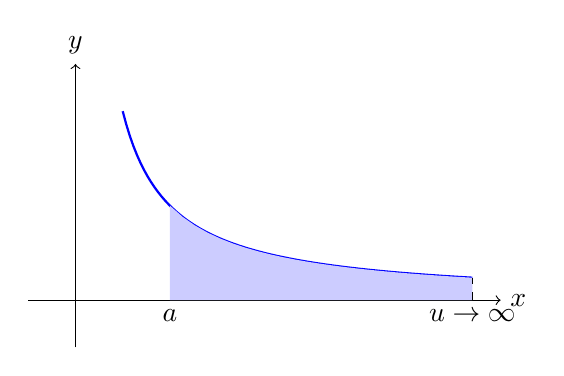
\begin{tikzpicture}[scale=1.2]
    \draw[->] (-0.5,0) -- (4.5,0) node[right] {$x$};
    \draw[->] (0,-0.5) -- (0,2.5) node[above] {$y$};
    \draw[thick, blue, samples=100, domain=0.5:4.2] plot (\x, {1/\x});
    \fill[blue!20, domain=1:4.2] (1,0) -- (1,1) -- plot (\x, {1/\x}) -- (4.2,0) -- cycle;
    \draw[dashed] (4.2,0) -- (4.2, {1/4.2});
    \node[below] at (1,0) {$a$};
    \node[below] at (4.2,0) {$u \to \infty$};
\end{tikzpicture}
\caption{无穷区间积分的示意图}
\end{figure}

类似地，可以定义其他无穷区间上的积分：
\[
\int_{-\infty}^{b}f(x)dx=\lim_{u\to -\infty}\int_u^b f(x)dx,
\]
\[
\int_{-\infty}^{+\infty}f(x)dx=\int_{-\infty}^{c}f(x)dx+\int_c^{+\infty}f(x)dx.
\]
对从 $-\infty$ 到 $+\infty$ 的积分，必须要求两个组成积分\textbf{分别}收敛。分割点 $c$ 的选择不影响收敛性。

\subsubsection{基准：$p$-积分（第一类）}
为了判断复杂函数的收敛性，经常把它们与幂函数 $1/x^p$ 比较。

\begin{theorem}
积分 $\int_1^{+\infty}\frac{1}{x^p}\,dx$：
\begin{itemize}
    \item 当 $p>1$ 时\textbf{收敛}；
    \item 当 $p\le 1$ 时\textbf{发散}。
\end{itemize}
\end{theorem}
\begin{proof}
计算 $\int_1^u x^{-p}\,dx$：
\begin{itemize}
    \item 如果 $p=1$，则 $\ln u\to\infty$，当 $u\to\infty$；
    \item 如果 $p\ne 1$，结果为 $\frac{u^{1-p}-1}{1-p}$。为了收敛，需要 $u^{1-p}\to 0$，这要求 $1-p<0$，即 $p>1$。
\end{itemize}
\end{proof}

\subsection{第二类反常积分（无界函数）}

这类积分出现在有限区间 $[a,b]$ 上，但被积函数 $f(x)$ 在一个或多个点处趋于无穷（有奇点）。

\begin{definition}
如果 $f$ 在 $[a,b)$ 上连续，但在 $b$ 处不连续（例如 $\lim_{x\to b^-}|f(x)|=\infty$），定义
\[
\int_a^b f(x)\,dx=\lim_{\epsilon\to 0^+}\int_a^{b-\epsilon}f(x)\,dx.
\]
\end{definition}

\subsubsection{基准：$p$-积分（第二类）}
注意：奇点情形下的收敛条件与无穷区间情形\textit{相反}。

\begin{theorem}
在区间 $(0,1]$ 上，积分 $\int_0^1\frac{1}{x^p}\,dx$：
\begin{itemize}
    \item 当 $p<1$ 时\textbf{收敛}；
    \item 当 $p\ge 1$ 时\textbf{发散}。
\end{itemize}
\end{theorem}

\subsection{收敛性的一般理论}

在应用实用判别法之前，先建立收敛的严格充要条件。

\subsubsection{Cauchy 准则}
Cauchy 准则很基础，因为它允许在不知道极限值的情况下证明收敛。

\begin{theorem}[反常积分的 Cauchy 准则]
积分 $\int_a^{+\infty}f(x)\,dx$ 收敛，\textbf{当且仅当} 对任意 $\epsilon>0$，存在 $M>a$，使得对所有 $u_2>u_1>M$，都有
\[
\left|\int_{u_1}^{u_2}f(x)\,dx\right|<\epsilon.
\]
\end{theorem}

\subsubsection{绝对收敛与条件收敛}
\begin{itemize}
    \item \textbf{绝对收敛：}$\int |f(x)|\,dx$ 收敛；
    \item \textbf{条件收敛：}$\int f(x)\,dx$ 收敛，但 $\int |f(x)|\,dx$ 发散。
\end{itemize}
\begin{theorem}
如果 $\int_a^{+\infty}|f(x)|\,dx$ 收敛，则 $\int_a^{+\infty}f(x)\,dx$ 收敛。
\end{theorem}

\subsection{收敛判别法}

\subsubsection{直接比较判别法}
\begin{theorem}
设 $f(x)$ 和 $g(x)$ 是 $[a,+\infty)$ 上的连续函数，且对所有 $x\ge a$ 有 $0\le f(x)\le g(x)$。
\begin{enumerate}
    \item 如果 $\int_a^{+\infty}g(x)dx$ 收敛，则 $\int_a^{+\infty}f(x)dx$ 也收敛。
    \item 如果 $\int_a^{+\infty}f(x)dx$ 发散，则 $\int_a^{+\infty}g(x)dx$ 也发散。
\end{enumerate}
\end{theorem}
\textit{直觉：}如果较大曲线下的面积有限，那么较小曲线下的面积也有限；如果较小曲线下的面积无限大，那么较大曲线下的面积必然无限大。

\begin{example}
$\int_1^{+\infty}\frac{\sin^2x}{x^2}dx$ 是否收敛？
\end{example}
\textbf{解：}因为 $0\le \sin^2x\le 1$，所以
\[
0\le \frac{\sin^2x}{x^2}\le \frac{1}{x^2}.
\]
已知 $\int_1^{+\infty}\frac{1}{x^2}dx$ 收敛（$p=2>1$）。由直接比较判别法，$\int_1^{+\infty}\frac{\sin^2x}{x^2}dx$ 收敛。

\subsubsection{极限比较判别法}

有时很难找到直接不等式。极限比较判别法通常更有力。

\begin{theorem}
设 $f(x)$ 和 $g(x)$ 是 $[a,+\infty)$ 上的正连续函数。如果
\[
\lim_{x\to +\infty}\frac{f(x)}{g(x)}=L,
\]
其中 $0<L<+\infty$，则 $\int_a^{+\infty}f(x)dx$ 与 $\int_a^{+\infty}g(x)dx$ 同敛散。
\end{theorem}
如果 $L=0$ 且 $g(x)$ 对应积分收敛，则 $f(x)$ 对应积分收敛；如果 $L=+\infty$ 且 $g(x)$ 对应积分发散，则 $f(x)$ 对应积分发散。

\begin{example}
分析 $\int_1^{+\infty}\frac{x}{1+x^3}dx$。
\end{example}
\textbf{解：}当 $x$ 很大时，常数项 $1$ 可忽略，因此
\[
\frac{x}{1+x^3}\approx \frac{x}{x^3}=\frac{1}{x^2}.
\]
令 $f(x)=\frac{x}{1+x^3}$，$g(x)=\frac{1}{x^2}$。则
\[
\lim_{x\to +\infty}\frac{f(x)}{g(x)}=\lim_{x\to +\infty}\frac{x/(1+x^3)}{1/x^2}=\lim_{x\to +\infty}\frac{x^3}{1+x^3}=1.
\]
由于 $L=1$（有限且为正），并且 $\int_1^{+\infty}\frac{1}{x^2}dx$ 收敛，所以原积分收敛。

对正函数使用比较判别法；对振荡函数，则需要更高级的工具。

\subsubsection{Cauchy 极限比较判别法（阶分析）}
这是判断收敛性最实用的方法。它形式化了把函数与 $1/x^p$ 比较的想法。

\begin{theorem}
设 $f(x)$ 是定义在 $[a,+\infty)$ 上的正函数。考虑 $f(x)$ 乘以测试幂 $x^p$ 后的极限：
\[
\lambda=\lim_{x\to +\infty}x^p f(x).
\]
\begin{enumerate}
    \item \textbf{收敛情形：}如果可以找到 $p>1$，使得 $0\le \lambda<+\infty$，则 $\int_a^{+\infty}f(x)\,dx$ \textbf{收敛}。
    \textit{含义：$f(x)$ 趋于零的速度快于 $1/x$，大致像 $1/x^p$。}
    \item \textbf{发散情形：}如果可以找到 $p\le 1$，使得 $0<\lambda\le +\infty$，则 $\int_a^{+\infty}f(x)\,dx$ \textbf{发散}。
    \textit{含义：$f(x)$ 趋于零的速度慢于或等于 $1/x$。}
\end{enumerate}
\end{theorem}

\begin{example}
检验 $\int_1^{+\infty}\frac{\ln x}{x^2}\,dx$。
由于 $x^2$ 占优，可以猜测收敛。取 $p=1.5$（因为 $1<1.5<2$，留出比较空间）：
\[
\lim_{x\to +\infty}x^{1.5}\frac{\ln x}{x^2}=\lim_{x\to +\infty}\frac{\ln x}{x^{0.5}}=0\quad (\text{由 L'Hôpital 法则}).
\]
因为 $p=1.5>1$ 且极限有限，所以积分收敛。
\end{example}

\subsubsection{Dirichlet 与 Abel 判别法（用于条件收敛）}
这些判别法用于乘积形式的积分 $\int_a^{+\infty}f(x)g(x)\,dx$，通常其中一部分振荡，另一部分衰减。

\begin{theorem}[Dirichlet 判别法]
积分 $\int_a^{+\infty}f(x)g(x)\,dx$ 收敛，如果：
\begin{enumerate}
    \item $f(x)$ 的部分积分有界：存在 $M$，使得对所有 $u>a$，$|\int_a^u f(t)\,dt|\le M$；
    \item $g(x)$ 单调递减，且 $\lim_{x\to +\infty}g(x)=0$。
\end{enumerate}
\end{theorem}
\textit{经典应用：}$\int_0^{+\infty}\frac{\sin x}{x}\,dx$。这里 $f(x)=\sin x$（积分有界），$g(x)=1/x$（单调趋于 $0$）。

\begin{theorem}[Abel 判别法]
积分 $\int_a^{+\infty}f(x)g(x)\,dx$ 收敛，如果：
\begin{enumerate}
    \item $\int_a^{+\infty}f(x)\,dx$ 收敛；
    \item $g(x)$ 单调且有界。
\end{enumerate}
\end{theorem}

\subsubsection{Cauchy 主值（P.V.）}

在某些发散积分中，如果以对称方式取极限，正负面积可能相互抵消。这个值称为 Cauchy 主值。

\begin{definition}
\begin{enumerate}
    \item 对 $c\in(a,b)$ 处的奇点：
    \[
    \text{P.V.}\int_a^b f(x)\,dx=\lim_{\epsilon\to 0^+}\left(\int_a^{c-\epsilon}f(x)\,dx+\int_{c+\epsilon}^{b}f(x)\,dx\right).
    \]
    \item 对无穷区间 $(-\infty,+\infty)$：
    \[
    \text{P.V.}\int_{-\infty}^{+\infty}f(x)\,dx=\lim_{R\to +\infty}\int_{-R}^{R}f(x)\,dx.
    \]
\end{enumerate}
\end{definition}

\begin{remark}
\textbf{收敛 $\implies$ 主值存在}，但反过来不成立。
\end{remark}

\begin{example}
考虑 $f(x)=\frac{1}{x}$ 在 $[-1,1]$ 上的积分。
\begin{itemize}
    \item \textbf{反常积分：}
    \[
    \int_{-1}^{1}\frac{1}{x}\,dx=\int_{-1}^{0}\frac{1}{x}\,dx+\int_0^1\frac{1}{x}\,dx.
    \]
    由于 $\int_{\epsilon}^{1}\frac{1}{x}\,dx=-\ln\epsilon\to\infty$，标准反常积分\textbf{发散}。
    \item \textbf{主值：}
    \[
    \text{P.V.}\int_{-1}^{1}\frac{1}{x}\,dx=\lim_{\epsilon\to 0^+}\left(\int_{-1}^{-\epsilon}\frac{1}{x}\,dx+\int_{\epsilon}^{1}\frac{1}{x}\,dx\right)=0.
    \]
    这是由函数的奇对称性造成的。
\end{itemize}
\end{example}

\subsubsection{综合例子：Gamma 函数}
\[
\Gamma(s)=\int_0^{+\infty}x^{s-1}e^{-x}\,dx.
\]
这个积分需要同时分析零点附近的奇性和无穷远处的行为。
\begin{itemize}
    \item \textbf{在 $0$ 附近：}如果 $s<1$，$x^{s-1}$ 有奇性。由于 $e^{-x}\approx 1$，它的行为类似于 $\int_0^1\frac{1}{x^{1-s}}dx$。由第二类 $p$-积分判别法，它在 $1-s<1$，即 $s>0$ 时收敛。
    \item \textbf{在 $+\infty$ 处：}$e^{-x}$ 的衰减快于任意幂 $x^p$ 的增长。用 $1/x^2$ 作极限比较：
    \[
    \lim_{x\to\infty}x^2(x^{s-1}e^{-x})=0.
    \]
    因而在无穷远处对所有 $s$ 都收敛。
\end{itemize}
\textbf{结论：}该积分在 $s>0$ 时收敛。

在本章最后，用所学知识解决一个有趣问题：Gabriel 号角。

考虑有一个号角，其横截面是圆，而纵截面由函数 $y=\frac{1}{x}$，$x\in(1,\infty)$ 描述。

先计算号角的体积：
\[
V=\pi\int_1^{+\infty}\left(\frac{1}{x}\right)^2dx=\pi\left[-\frac{1}{x}\right]_1^{+\infty}=\pi.
\]
可以看到，这个号角有有限体积。

再计算其表面积：
\[
S=2\pi\int_1^{+\infty}\frac{1}{x}\sqrt{1+\frac{1}{x^4}}dx\ge 2\pi\int_1^{+\infty}\frac{1}{x}dx=+\infty.
\]
表面积对应的积分发散。

这里出现了一个非常有趣的悖论：可以用有限多的油漆填满这个号角，但这桶油漆却无法涂满号角的内壁。

这个结果与我们的朴素理解相矛盾。

本章结束时要记住：这不是终点，而是一道入口。数学分析的旅程还会继续。在\textbf{第 4 章}中，我们会把这些基础扩展到更高维，进一步研究曲线和曲面，并遇到更多优美而出人意料的结果。这个来自无穷领域的号角之声，邀请我们继续探索。

在后续章节中，我们还会进入更多分析学高级主题，例如多变量微积分、微分方程、复分析和泛函分析。每一个领域都建立在本章发展的概念之上，并各自带来独特的洞见与挑战。希望读者带着本章获得的严谨工具和深入理解，继续探索下去。

\vspace{1cm}
\noindent
\textbf{参考文献：} \\
Mathematical Analysis (Third Edition), Chen, J., Higher Education Press \\
The Real Numbers and Real Analysis, Ethan D. Bloch, Springer

\cleardoublepage
